
\documentclass[a4paper,12pt]{article}
% --------------------------


% 0.1. -- Add packages --
\usepackage{amsmath,amssymb,amsthm}
\usepackage{graphicx}
\graphicspath{{../Figures/}{../Results/Figures/}{./}}
\usepackage{mathtools}
\usepackage{comment}
\usepackage{amsfonts}
\usepackage{bbm,bm}
\usepackage{physics}
\usepackage{float}
\usepackage{cancel}
\usepackage{cases}
\usepackage{ascmac}
\usepackage{ulem} 
\usepackage[english]{babel}
\usepackage[hang,flushmargin]{footmisc}
\usepackage{stmaryrd}
\usepackage{booktabs}
\usepackage[top=25truemm,bottom=25truemm,left=20truemm,right=20truemm]{geometry}
\usepackage{setspace}
\overfullrule = 0pt % mute overfull box
% --------------------------
% (note) you can add other packages which you wanna use by typing "\usepackage{[package name]}"
\usepackage{tikz}

\usepackage[hidelinks]{hyperref}
\usepackage{siunitx}

\usepackage[authoryear,round]{natbib}
\bibliographystyle{chicagoa}

\usepackage{subcaption}
\usepackage{makecell}
 \linespread{1.2}

\makeatletter
\def\input@path{{./sections/}{./appendix/}{../Results/Tables/}{./}}
\makeatother
% 0.2. -- define new commands (example) --
\newcommand{\latex}{\LaTeX~}
\newcommand{\define}{\overset{{\rm def }}{\Leftrightarrow}}
\newcommand{\C}{\mathbb{C}}
\newcommand{\R}{\mathbb{R}}
\newcommand{\N}{\mathbb{N}}
\newcommand{\Q}{\mathbb{Q}}
\newcommand{\Z}{\mathbb{Z}}
\newcommand{\F}{\mathcal{F}}
\newcommand{\argmax}{\mathop{\rm arg~max}\limits}
\newcommand{\argmin}{\mathop{\rm arg~min}\limits}
\newcommand{\vin}{\rotatebox{90}{$\in$}}
% --------------------------
% (note) you can define new command to shorten the code. Please Google or create by yourself and add as needed.


% 0.3. -- setting for Matlab code --
\usepackage{listings}
\lstset{
    language=Matlab,
	basicstyle={\ttfamily},
	identifierstyle={\small},
	commentstyle={\smallitshape},
	keywordstyle={\small\bfseries},
	ndkeywordstyle={\small},
	stringstyle={\small\ttfamily},
	frame={tb},
	breaklines=true,
	columns=[l]{fullflexible},
	numbers=left,
	xrightmargin=0ex,
	xleftmargin=3ex,
	numberstyle={\scriptsize},
	stepnumber=1,
	numbersep=1ex,
	lineskip=-0.5ex
}
\usepackage[T1]{fontenc} %change font encoding to T1
\usepackage[framed,numbered]{matlab-prettifier}

\title{When Monitoring Backfires: Multi-Tasking Bureaucrats and Land Misallocation in China
\footnote{I am grateful to Yasuyuki Sawada, and all seminar participants at the University of Tokyo, and conference participants at Young JADE, for their illustrative guides and comments. I acknowledge the assistance of GPT 5.2 in proofreading the draft of this
paper. All errors are my own.}}



\date{\today}


\author{
    Ze Wang\thanks{The University of Tokyo. wangze@g.ecc.u-tokyo.ac.jp}
}


\begin{document}

\maketitle

\centerline{\color{blue}\href{https://www.dropbox.com/scl/fi/ex67w501hojuiegcu77yn/ZeWang_Cropland.pdf?rlkey=5c99k5iqay90ucazea5qi2c0s&dl=0}{Latest version available here} \color{black}}

\centerline{This is a work-in-progress paper.}

\begin{abstract}
    This paper examines how strengthened enforcement of performance targets affects policy implementation when local officials face multitask incentives and imperfect monitoring. I examine China’s 2017 tightening of cropland protection, which made compliance with cropland-area targets a binding component of bureaucratic evaluations while leaving land quality and utilization weakly monitored. Exploiting cross-county variation in cropland protection pressure arising from differential exposure to binding cropland constraints within prefectures, I combine high-resolution satellite data on land cover, soil suitability, and vegetation dynamics to trace land-use responses at a fine spatial scale. I find that stricter enforcement increases cropland expansion in high-pressure counties, yet the land brought into cultivation is of lower agronomic quality and displays persistently higher fallow rates. These effects are stronger when officials face higher promotion incentives and heavier economic growth pressures. The results show that strengthening oversight along observable dimensions can induce distortions along less observable ones, generating land misallocation and productivity losses.
\end{abstract}


\pagebreak

\section{Introduction}
Governments in centralized administrative systems have to rely on delegation and incentive contracts to implement national goals \citep{williamson1985economic}. However, asymmetric information between upper-level and local governments, combined with the fact that local officials face promotion incentives tied to performance across multiple tasks such as promoting economic growth while meeting environmental protection requirements, can lead to deviations from policy objectives \citep{holmstrom1991multitask, chen2018career}. A common response from the center is to strengthen monitoring and performance-based assessments in an effort to narrow information gaps and realign local incentives embedded in these contracts. Yet when monitoring remains incomplete and is observable on some dimensions but not others, tighter supervision raises the possibility that distortions may be shifted rather than eliminated.

When the center tightens supervision over dimensions it can readily observe, does this induce distortions along dimensions that remain imperfectly monitored? This paper addresses this question by studying China’s tightening of cropland protection policy and its implications for local officials’ land allocation choices. Specifically, I examine whether stricter enforcement of cropland quantity targets reshapes the trade-off local governments face between allocating land to urban expansion, which supports economic growth, and allocating land to cropland to satisfy binding protection requirements.

Local governments in China have long been evaluated primarily on economic performance, particularly economic growth \citep{fan2025land}. To support industrialization and urban expansion, local officials have strong incentives to convert land for construction use, making land allocation a central instrument of local development policy. At the same time, concerns over food security prompted the central government to introduce the “red line” cropland protection policy in the early 2000s, which mandates a minimum national cropland area.\footnote{The red line policy stipulates that total arable land should remain no less than 120 million hectares, reflecting national concerns over grain self-sufficiency.} Local governments thus operate in a multitask environment that requires balancing economic development with cropland protection.

Prior to 2017, however, cropland protection was weakly enforced despite the formal existence of quantitative targets. This changed with the 2017 reform of the cropland protection responsibility assessment system, under which compliance with cropland protection targets became a binding component of official evaluations and promotion criteria. While the reform aimed to strengthen the joint management of cropland quantity and productive capacity, in practice enforcement focused almost exclusively on observable cropland quantity. Monitoring of cropland quality and subsequent utilization remained limited. This asymmetry raises a key concern: when quantitative targets become binding under incomplete monitoring, local governments may comply by expanding cropland area through the reclamation of marginal or low-quality land, generating distortions in land allocation.

In this paper, I use satellite-based raster data to identify cropland and cultivation intensity. The unit of observation is a $500 \times 500$ meter grid cell. Aggregating raster measures to the grid level allows me to track changes in land allocation and land use at a spatial scale relevant for local policy implementation, while avoiding reliance on administrative statistics that may be subject to reporting biases.

I leverage cross-county exogenous variation in cropland protection pressure to identify the effects of tighter cropland protection on land allocation and cultivation outcomes. Cropland protection pressure captures the extent to which local governments are constrained in meeting cropland protection requirements given ongoing land conversion demands. It arises from institutional features of China’s cropland occupation--replenishment system, which allow replenishment obligations to be met outside the converting county. In cases where a county or district lacks sufficient land, replenishment is, in principle, arranged through cross-county adjustment within the same prefecture, with available land across the prefecture serving as a shared reservoir.

As a result, counties differ in their exposure to binding cropland protection constraints depending on their relative endowment of available land within the prefecture. Prefecture-level cropland obligations act as a common policy shock, while pre-existing county-level land endowments determine differential exposure. This institutional structure generates plausibly exogenous variation in cropland protection pressure, which the analysis exploits to study how stricter enforcement reshapes land-use decisions and cultivation outcomes.

This study finds that tighter enforcement of cropland protection affects land-use decisions along both the extensive and intensive margins of land use. On the extensive margin, counties facing greater cropland protection pressure respond more strongly to the post-2017 assessments, with grid cells becoming significantly more likely to be converted into cropland. On the intensive margin, however, cropland reclaimed after the policy in high-pressure counties tends to be of lower soil suitability and is less likely to be actively cultivated, exhibiting higher fallow rates in subsequent years. Further analysis points to multitask incentives as a key mechanism: when promotion incentives are strong, and officials face heightened pressure to balance economic growth with cropland protection, compliance with binding quantity targets is achieved more through the reclamation of low-quality land. Although the policy tightening was intended to realign local implementation with central objectives, the evidence suggests that land misallocation and inefficiency can arise in practice when monitoring of land quality and utilization remains incomplete.

This study contributes to several strands of the literature. First, it is closely related to the multitasking principal–agent framework \citep{holmstrom1991multitask, baker1992incentive}. In contrast to a large empirical literature that examines how governments trade off opposing tasks in the Chinese context \citep{hong2025order, fan2025land, chen2018career, he2020watering}, this paper shifts attention to within-task distortions under imperfect monitoring. It provides the first empirical evidence that stricter performance measures may backfire when oversight is incomplete. Moreover, the existing multitasking literature has largely focused on the balance between environmental and economic objectives. To the best of my knowledge, this paper is the first to examine multitasking incentives in land-use regulation, thereby contributing to the broader literature on land regulation \citep{cai2017build, hilber2016impact, besley2000land}.

This study also contributes to the literature on misallocation and agricultural productivity \citep{adamopoulos2022misallocation, restuccia2017land, lagakos2013selection}. While \cite{adamopoulos2022misallocation} links misallocation in China to distortionary policies, their analysis focuses on productivity losses arising from misallocation across agricultural production factors. By contrast, this paper shows how imperfect performance evaluation systems can generate land misallocation across land-use types, highlighting a distinct channel through which policy-induced distortions affect agricultural efficiency.

Finally, this paper contributes to the literature on the political economy of the Chinese economy. A large body of work emphasizes that the central government frequently relies on top-down planning and performance-based mandates to implement nationwide policies, yet implementation outcomes often deviate from central objectives due to policy design constraints, information asymmetries, or strategic behavior by local governments \citep{wang2025policy, FismanWangYe2025_StrategicCaptureOfMonitors, axbard2024informed, henderson2022political}. Existing studies primarily focus on the logic of policy design, the role of information transmission, or the emergence of collusion. This paper adds to this strand of literature by showing how implementation distortions can arise even in the absence of collusion or explicit manipulation. When local governments face binding multitask incentives under imperfect monitoring, policy compliance along observable dimensions can naturally generate resource misallocation and productivity losses along less observable ones.

The remainder of the paper is organized as follows. Section~\ref{sec:background} describes the institutional background in China, with a focus on cropland protection policy. Section~\ref{sec:data} presents the data and explains the construction of the cropland protection pressure measure. Section~\ref{sec:fact} documents a set of motivating facts. Section~\ref{sec:concept} introduces a conceptual framework that guides the empirical analysis. Section~\ref{sec:empirical} presents the empirical strategy and main results. Section~\ref{sec:conclude} concludes.


\section{Institutional Background\label{sec:background}}
\subsection{Cropland Protection Policy and the Requisition--Compensation Balance System}

To ensure food security and agricultural self-sufficiency, the Chinese government enforces a cropland protection policy that requires the total area of cropland to remain stable over time. This aggregate quantity constraint, commonly referred to as the ``cropland red line``, mandates that the national cropland area not decline, conditional on no deterioration in overall land quality (\cite{StateCouncil2006NationalLandUsePlan_EN}).

The implementation of the cropland protection policy relies on a quota-based system embedded in China’s administrative hierarchy. The central government first sets a national cropland retention target, which is subsequently allocated to provincial governments. Provincial authorities further disaggregate these targets to prefecture- and county-level jurisdictions. As a result, each local government is assigned a binding cropland quota that it is responsible for fulfilling.

Maintaining this aggregate cropland target becomes particularly challenging in the context of rapid industrialization and urban expansion, especially in jurisdictions with rapid urban expansion. To reconcile urban development with cropland protection, the central government introduced the \emph{requisition--compensation balance system}(\cite{StateCouncil1998LandAdminRegulations}). Under this policy, any reclamation of cropland for non-agricultural use must be offset by the replenishment of an equivalent amount of new cropland, thereby preserving cropland quantity at the aggregate level.

In practice, local governments are granted limited flexibility in meeting these quotas through spatial adjustment. When a county is unable to achieve the requisition--compensation balance within its own jurisdiction, it may adjust cropland quotas with neighboring counties within the same prefecture. If such an adjustment remains infeasible, cross-county compensation can be arranged within the province among areas with comparable resource endowments. Through these within-jurisdiction adjustments, the policy aims to maintain aggregate cropland quantity while accommodating heterogeneity in local land conversion pressures.

\begin{figure}[htbp]
\begin{center}
  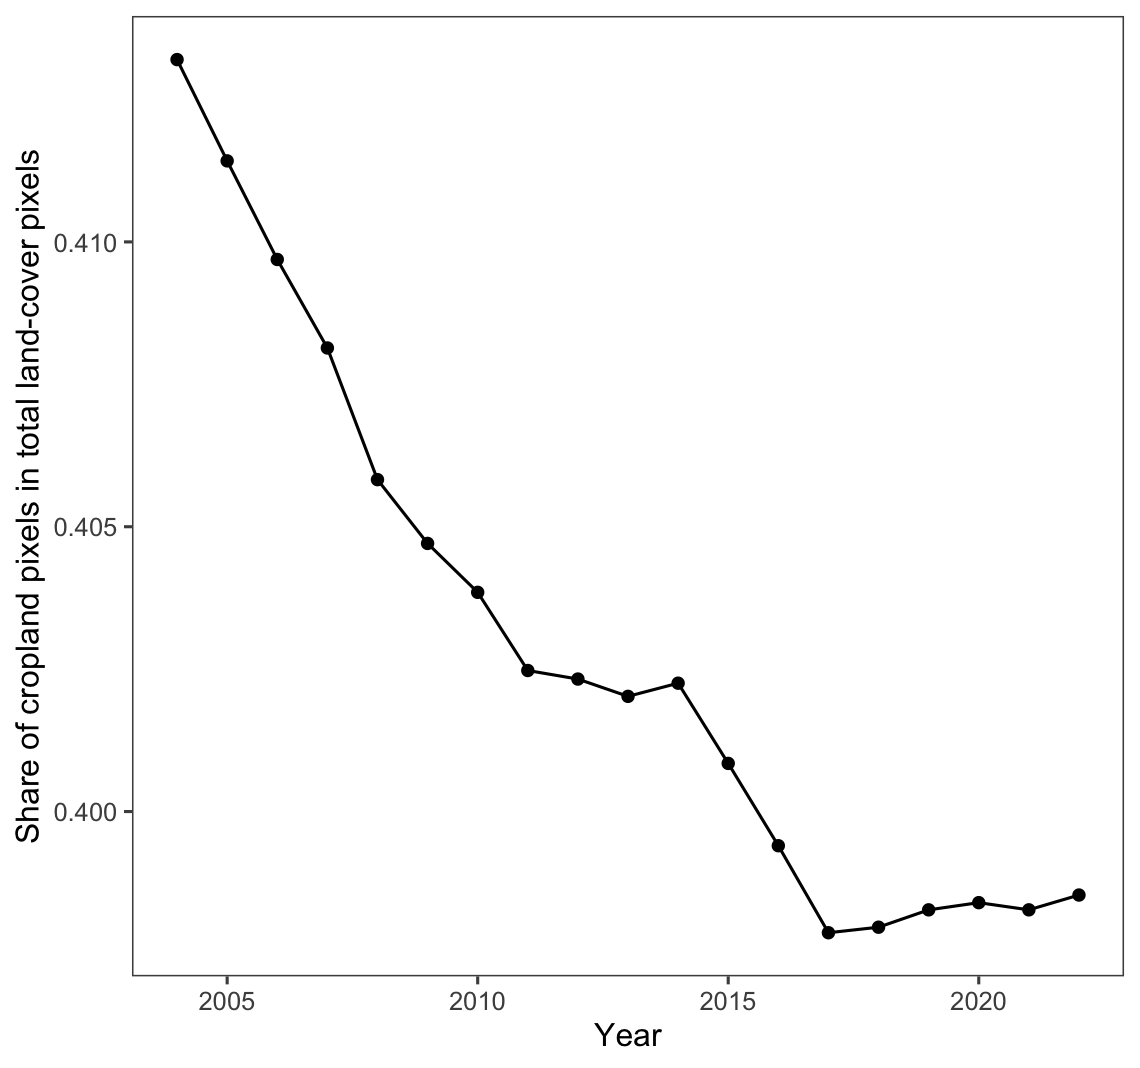
\includegraphics[width=0.6\textwidth]{background_crop_1.png}
\caption{Changes in Cropland Share in China}
\label{fig:landuse}
\end{center}
\footnotesize Data Source: China Land Cover Data.
\end{figure}

\subsection{Policy Revision and Monitoring Tightening in 2017}

Cropland protection has been a long-standing policy priority in China since the early 2000s. The State Council has imposed binding targets on cropland retention, requiring each administrative jurisdiction to maintain cropland area above an assigned benchmark. In practice, however, enforcement of these targets remained weak prior to 2017, potentially due to monitoring difficulties and an underdeveloped accountability system. As illustrated in Figure~\ref{fig:landuse}, the national share of cropland continued to decline steadily between 2005 and 2017, despite the existence of formal protection targets.

In order to strengthen the implementation of the requisition--compensation balance system and reinforce the cropland red line, the State Council issued the \textit{Opinions on Strengthening Cropland Protection and Improving the Requisition--Compensation Balance System}\footnote{\cite{CPCStateCouncil2017farmland}} in 2017 (hereafter, the 2017 Opinions). The 2017 Opinions revised the existing cropland protection framework by enhancing responsibility assignment and tightening monitoring mechanisms. In particular, while principal leaders of local governments at all administrative levels had long been identified as the first responsible persons for cropland protection, the 2017 Opinions further strengthened this responsibility by explicitly linking cropland protection performance to official evaluations, including cadre performance assessments and assessments related to ecological civilization construction.

The revised policy was implemented through a top-down governance structure. As shown in Figure~\ref{fig:timeline}, following the issuance of the 2017 Opinions by the central government in January 2017, a formal assessment framework for provincial governments was promulgated in January 2018. Provincial governments subsequently adopted corresponding responsibility assessment measures for lower-level jurisdictions, thereby cascading the strengthened protection requirements downward through the administrative hierarchy.

The stated objective of the 2017 policy revision was to establish a new cropland protection mechanism that emphasizes both quantity and productive capacity. On the quantity dimension, national cropland area stabilized after 2017 and exhibited a modest recovery, as shown in Figure~\ref{fig:landuse}. On the quality and productive capacity dimension, however, outcomes appear less clear-cut. Although the central government introduced monitoring systems intended to track cropland quality, ex post evidence suggests limited effectiveness. Reports by official media in the post-2017 period document persistent concerns regarding newly created cropland, including low land quality, abandonment, and subsequent loss \citep{Wang2023balance}. These accounts often attribute such outcomes to misaligned incentives and insufficient coordination across cropland protection policies and implementation measures.

\begin{figure}
    \centering
    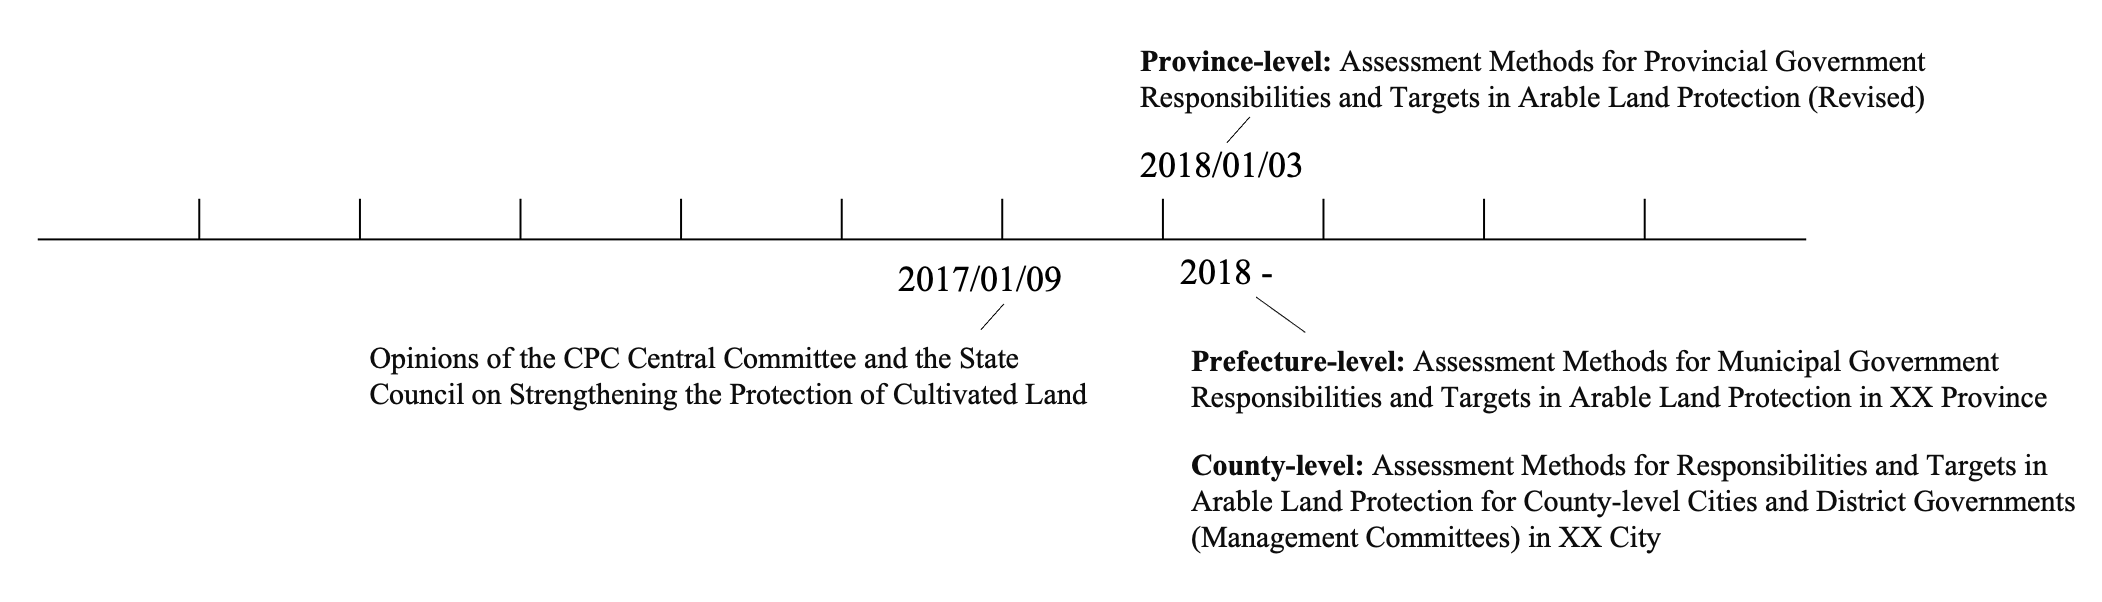
\includegraphics[width=0.85\linewidth]{timeline.png}
    \caption{Timeline}
    \label{fig:timeline}
\end{figure}

\subsection{Jiangsu Province}

This study focuses on Jiangsu Province rather than conducting a nationwide analysis. The objective of the paper is to examine land misallocation and inefficient land use arising from multitask pressures faced by local governments, specifically the tension between economic development and cropland protection. Although cropland protection targets are formally imposed nationwide, they do not constitute a binding constraint in all provinces. In regions with relatively slow urbanization, weak economic growth pressure, persistent population outflows, or abundant land reserves, local governments face limited trade-offs between urban expansion and cropland retention. In such settings, the multitask incentives central to this study are unlikely to arise in a meaningful way.

Jiangsu provides a particularly suitable empirical setting for studying these trade-offs. It is one of China’s most economically developed provinces, with among the highest levels of GDP per capita and a long history of rapid urbanization. Located in the Yangtze River Delta, Jiangsu is characterized by flat terrain and a high share of land suitable for cultivation, which has historically supported intensive agricultural production. At the same time, sustained industrialization and urban expansion generate strong and persistent demand for construction land. As a result, local officials in Jiangsu face especially acute conflicts between meeting economic development objectives and complying with binding cropland protection targets, a tension that is repeatedly emphasized in provincial and central government policy documents. 

%(\textcolor{blue}{TBD 江苏省土地利用总体规划})


\section{Data and Measurement\label{sec:data}}
\subsection{Data Sources and Measurement}

This study primarily relies on satellite-based raster data to measure land characteristics at a fine spatial resolution. To harmonize datasets with different spatial and temporal resolutions and to facilitate empirical analysis, I overlay all raster layers onto a uniform $500 \times 500$ meter grid covering the study area. For each grid cell, I compute average values of the underlying raster measures, which constitute the main unit of observation in the analysis.

\begin{table}[h]
    \centering
    
\begin{tabular}{p{6cm} p{8cm}}
\toprule
\textbf{Data Type} & \textbf{Source} \\
\midrule
Land Cover and Cropland Dynamics 
& 30 m annual land cover dataset for China (2012--2022)\\
\\
Fractional Vegetation Cover (FVC) 
& 30 m, 15-day FVC dataset, National Tibetan Plateau Data Center \\
\\
Soil Characteristics 
& 1:1,000,000 Soil Map of China compiled by the National Soil Survey Office (1995) \\
\\
Bureaucrat Characteristics 
& Prefecture- and province-level officials collected from publicly available online biographies \\
\\
Administrative Boundaries 
& China county-level shapefiles from Harvard Dataverse \\
\\
Socioeconomic Variables 
& County Statistical Yearbooks \\
Cropland Replenishment Obligation 
& Prefecture Land Use Master Plan (2006 -2020) \\
\bottomrule
\end{tabular}


    \caption{Data Sources}
    \label{tab:datasource}
\end{table}

\subsubsection{Cropland}

As summarized in Table~\ref{tab:datasource}, cropland information is obtained from the 30-meter annual land cover dataset for China (CLCD; \cite{yang2021_30m_landcover_china}). The CLCD provides annual land cover classifications from 1990 to 2021 at a 30-meter resolution, distinguishing among cropland, forest, shrubland, grassland, barren land, impervious surface, water bodies, snow, and ice. This dataset allows me to identify both cropland and built-up areas, with the latter captured by the impervious surface category.

\subsection{Fractional Vegetation Cover and Measurement of Fallow Rate}

Fractional Vegetation Cover (FVC) data are obtained from the National Tibetan Plateau Data Center \citep{zhao2023fractional}. The original dataset provides spatiotemporally continuous vegetation cover for China at a 30-meter resolution and a bimonthly frequency from 2010 to 2022. Following standard practice in the remote sensing literature, I aggregate the bimonthly observations to annual averages at the grid-cell level, which serve as a measure of vegetation coverage for each grid-year.

I use FVC to measure land-use intensity and to define fallow land. A grid cell is classified as fallow in a given year if its annual average FVC is below 0.2, which corresponds to the bottom 25 percent of the FVC distribution across cropland grids. This threshold captures land with very low vegetation cover and limited cultivation activity. In Appendix Figure~\ref{fig:sensitivity_fallow02}, I examine the sensitivity of the results to alternative FVC cutoffs. The estimates remain stable when the threshold is chosen sufficiently low, indicating that the main findings are not driven by the specific choice of cutoff.


\subsection{Soil Type and Measurement of Soil Suitability}

Soil information is obtained from the 1:1,000,000 Soil Map of China compiled by the National Soil Survey Office in 1995. A potential limitation of this measure is that soil characteristics are time-invariant over the sample period. However, this feature is unlikely to pose a major concern for the analysis, since soil type reflects long-run geological and pedological conditions that evolve slowly over time and are largely predetermined with respect to recent policy changes. 

I measure land quality using a grid-level soil suitability index constructed from soil type classifications as shown in Table~\ref{tab:soilmap}. The mapping from soil types to suitability scores follows the FAO Land Evaluation Framework and China’s National Land Capability Standard (GB/T 28407–2012), which provides qualitative guidelines for assessing agricultural suitability based on soil properties. Because these frameworks do not offer a one-to-one correspondence between specific soil types and numerical suitability scores, the resulting index should be interpreted as a coarse proxy for inherent land quality rather than a precise agronomic measure.

Specifically, I assign each soil type a suitability score ranging from 1 to 5, corresponding to FAO suitability classes from permanently unsuitable to highly suitable, and compute the grid-level score as the average across soil types within each $500 \times 500$ meter grid cell. To facilitate interpretation and reduce sensitivity to the exact scoring scheme, I additionally classify land as suitable if the average score is at least 3, and unsuitable otherwise. This cutoff separates soils that are marginally suitable or better from soils that are saline, alkaline, waterlogged, or otherwise non-arable, which correspond to the lowest suitability classes. 

\begin{table}[h]
    \centering
    \caption{Mapping Soil Types to Suitability Classes}
    \begin{tabular}{l l l}
\hline
\textbf{Score} & \textbf{FAO Class} & \textbf{Representative Soil Groups} \\
\hline
5 (S1) & Highly suitable 
& Fluvisols, Anthrosols, alluvial soils \\
4 (S2) & Moderately suitable 
& Cambisols, Luvisols, Ferralsols, Andosols \\
3 (S3) & Marginally suitable 
& Regosols, Leptosols, Cambic soils, hardpan soils \\
2 (N1) & Currently unsuitable 
& Saline soils, sodic soils, waterlogged paddy soils \\
1 (N2) & Permanently unsuitable 
& Urban land, marsh soils, water bodies, sandbars \\
\hline
\end{tabular}
    \label{tab:soilmap}
\end{table}

\subsubsection{Administrative and Socioeconomic Data}

Administrative data on government officials are collected from publicly available online biographies. The dataset records key characteristics of prefecture- and province-level officials, including appointment and departure years, gender, age, and place of birth. County-level socioeconomic variables are obtained from the China County Statistical Yearbooks. The data include information on economic activity, agricultural production, population, and fiscal conditions. In addition, cropland replenishment obligations are collected from prefecture-level Land Use Master Plans, which specify each jurisdiction’s targets for urban expansion and cropland replenishment obligation through 2020.


\subsection{Measuring Land Protection Pressure}


This subsection constructs a county-level measure of exposure to binding cropland protection constraints. The measure captures the land protection pressure faced by local officials, which reflects the intensity of multitask pressure arising from the need to satisfy cropland protection targets while accommodating urbanization and development demands. It serves as the key explanatory variable in the empirical analysis. 

The construction of the land protection pressure measure exploits institutional features of China’s cropland occupation--replenishment system. Two policy rules are central to this design:

\begin{enumerate}
    \item \textbf{Cropland occupation--replenishment rule.} Any conversion of cropland to construction land must be offset by the creation of an equivalent amount of new cropland.
    
    \item \textbf{Non-local replenishment with prefecture-level priority.} Replenishment is not necessarily required to occur within the converting county. When core urban districts lack sufficient land, cropland replenishment is, in principle, fulfilled through \emph{cross-county adjustment within the same prefecture}. Only if prefecture-level adjustment is infeasible may replenishment be arranged across prefectures within the same province, typically through a paid transaction mechanism.
\end{enumerate}

Together, these rules imply that cropland replenishment is constrained by land availability at the prefecture level. Because core urban districts are primarily tasked with meeting economic growth targets, their cropland replenishment obligations are frequently met by counties within the same prefecture.\footnote{This practice is documented in official planning materials. For example, Lianyungang City’s Land Use Master Plan states that “districts such as Haizhou District and Lianyun District that are unable to achieve local farmland reclamation–replacement balance due to insufficient land reserves may, upon approval, implement off-site reclamation–replacement within the municipal jurisdiction, provided that the aggregate reclamation obligation remains unchanged.”} As a result, non-core counties serve as a shared land reservoir that absorbs replenishment obligations generated by urban expansion, creating variation in cropland protection pressure across counties.\footnote{The definition of the core urban area is specified in each prefecture’s Land Use Master Plan (2006–2020).}


Based on this structure, I define land protection pressure at the county level as
\begin{equation}
\text{Pressure}_{c}
=
\left(
\frac{\text{Obligation}_{p}}
     {\text{TotalLand}_{p}}
\right)
\times 
\text{LandShare}_{c},
\end{equation}
where $p$ denotes the prefecture to which county $c$ belongs. $\text{Obligation}_{p}$ measures the total cropland replenishment obligation assigned to the core urban districts of prefecture $p$ under provincial land-use planning targets. $\text{TotalLand}_{p}$ captures the total area of available land outside core urban districts within prefecture $p$, excluding impervious surfaces and water bodies, and represents the effective land reservoir for cropland replenishment. $\text{LandShare}_{c}$ denotes county $c$’s share of this reservoir, defined as the ratio of available land in county $c$ to the total available land summed across all non-core counties within the same prefecture.

This construction implies that counties with larger shares of non-core, available land are more exposed to cropland replenishment pressure when prefecture-level obligations increase. Importantly, $\text{LandShare}_{c}$ is determined by pre-existing land endowments and administrative boundaries, and is fixed prior to the tightening of cropland protection in 2017. As a result, conditional on prefecture-level obligations, cross-county variation in land protection pressure reflects an exogenous allocation of replenishment capacity rather than endogenous policy choices by county governments. Conceptually, this structure resembles a shift–share design, in which prefecture-level replenishment obligations act as the common shock, while county-level land shares determine differential exposure. This feature underpins the empirical strategy used in subsequent sections.

To assess the extent to which variation in $Pressure_c$ arises within prefectures, Figure~\ref{fig:box} plots the distribution of the pressure index across counties by prefecture. Each box summarizes the distribution of land protection pressure among non-core counties within a prefecture, with the thick horizontal line indicating the prefecture-level median. Differences in median pressure across prefectures capture between-prefecture variation, while the dispersion of observations within each box reflects within-prefecture heterogeneity in land protection pressure. The figure shows that the pressure index has sufficient variation both across and within prefectures.

\begin{figure}[htbp]
\centering
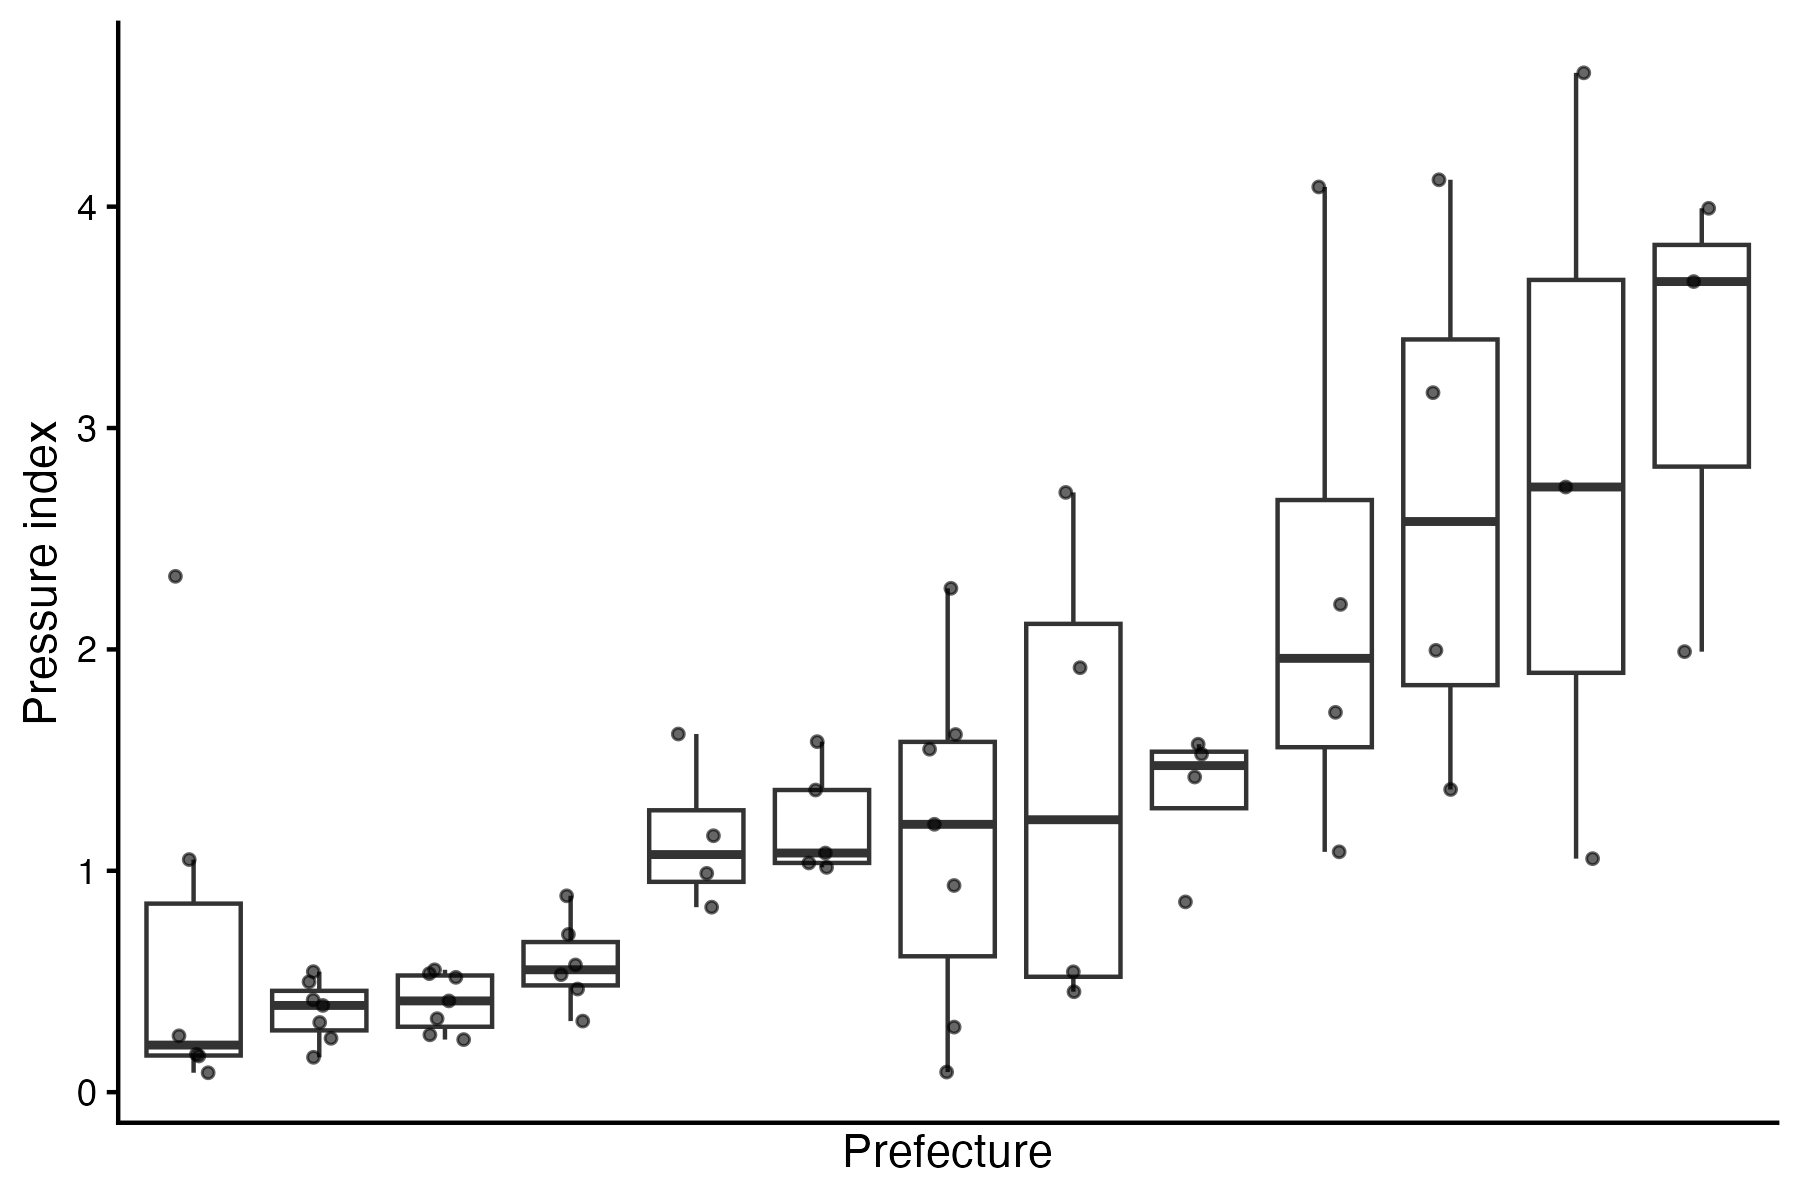
\includegraphics[width=0.8\linewidth]{Pressure_c_boxplot.png}
\caption{Distribution of Land Protection Pressure within and across Prefectures}
\caption*{\footnotesize \textit{Notes}: This figure plots the distribution of the land protection pressure index ($Pressure_c$) across counties within each prefecture. Each box summarizes the distribution of $Pressure_c$ among non-core counties within a prefecture: the box represents the interquartile range (25th–75th percentiles), and the thick horizontal line indicates the median. Dots denote individual counties.}
\label{fig:box}
\end{figure}

To formally distinguish the within- and between-prefecture components of variation in this key variable, I conduct a simple variance decomposition based on the ANOVA identity.\footnote{$
\sum_{c,p} \left( X_{cp} - \bar{X} \right)^2
=
\sum_{p} n_p \left( \bar{X}_p - \bar{X} \right)^2
+
\sum_{p} \sum_{c \in p} \left( X_{cp} - \bar{X}_p \right)^2 .$} Specifically, total variation in $Pressure_c$ is decomposed into variation across prefecture-level means and variation across counties within the same prefecture. The results indicate that 39.8\% of the total variation in the pressure index arises from within-prefecture differences across counties, while the remaining $60.2\%$ reflects differences across prefectures.


%\subsection{Summary Statistics}%

\section{Motivating Facts\label{sec:fact}}

\subsection{Land-Use Area Trends by Land Protection Pressure}

Descriptive analysis reveals a central contrast between high- and low-pressure prefectures. Following the 2017 tightening of cropland protection, urban expansion trajectories remain similar across prefectures, whereas cropland adjustment differs sharply by land protection pressure. Figure~\ref{fig:size} presents prefecture-demeaned trends in impervious surface area and cropland area, separately for core and non-core areas and by land protection pressure.

Across both core and non-core areas, trends in impervious surface expansion are broadly comparable between high- and low-pressure prefectures, with steady growth and no visible divergence around 2017. This pattern indicates that urban development proceeded along similar paths regardless of land protection pressure, in line with the continued prioritization of economic growth objectives.

In contrast, cropland dynamics diverge markedly by land protection pressure after 2017. Prior to the policy tightening, cropland area declines in both high- and low-pressure prefectures. After 2017, however, cropland area rebounds and increases in high-pressure prefectures, while continuing to decline and exhibiting only a limited and delayed recovery in low-pressure prefectures. This divergence is concentrated in non-core areas; cropland trends within core urban areas remain similar across prefecture types throughout the period.

These patterns suggest that the 2017 policy tightening primarily constrained high-pressure prefectures, while having limited effects in low-pressure prefectures. At the same time, urban expansion in core areas appears insulated from these constraints, implying that the burden of meeting binding cropland protection targets was shifted toward non-core areas within high-pressure prefectures.



\begin{figure}[h]
    \centering
    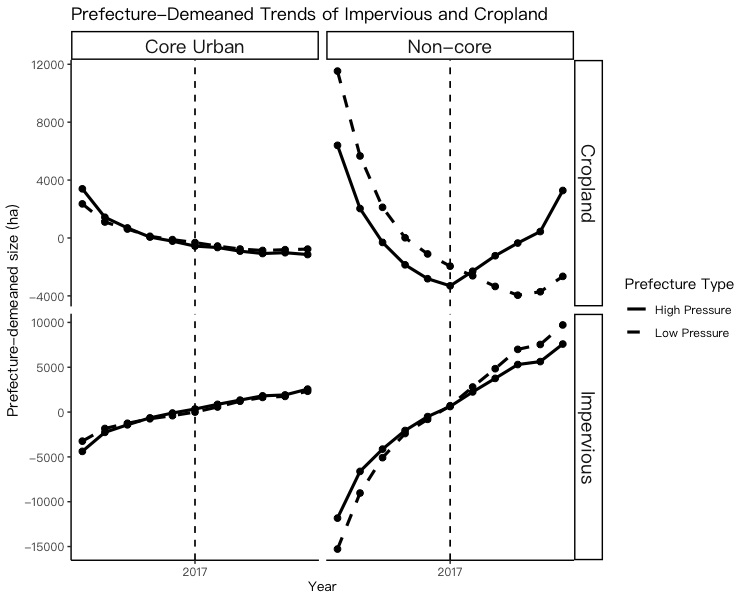
\includegraphics[width=0.8\linewidth]{Motivating_size.png}
    \caption{Trends in impervious area and cropland area by land type}
    \label{fig:size}
\end{figure}

\subsection{Vegetation Coverage over the Reclamation Cycle}

Figure~\ref{fig:fvc} illustrates the evolution of fractional vegetation coverage on newly reclaimed land as a function of years since reclamation. Pooling all newly reclaimed grids in the sample, mean FVC increases monotonically over time. This pattern indicates that vegetation coverage improves gradually following reclamation, indicating that FVC captures the intensity of agricultural use and land cultivation in the years after cropland creation.

Figure~\ref{fig:fvc_group} further disaggregates these patterns by land protection pressure and policy period. For grids reclaimed prior to 2018, as well as for grids located in low-pressure prefectures, FVC exhibits a similar upward trajectory to that observed in the full sample, increasing with years since reclamation. In contrast, newly reclaimed land in high-pressure prefectures after the policy tightening displays a markedly different pattern. These grids exhibit substantially lower initial FVC and show little subsequent improvement over time, with mean vegetation coverage remaining persistently low.

In a nutshell, these descriptive patterns suggest that while newly reclaimed land typically becomes increasingly cultivated over time, this process is disrupted for cropland created after the policy tightening in high-pressure prefectures. The persistently low vegetation coverage observed for these grids is consistent with a higher likelihood of underutilization or temporary fallow, whereas similar patterns are not observed in low-pressure prefectures. These motivating facts point to heterogeneous responses to the tightening of cropland protection, concentrated in regions where land protection constraints are most binding.


    \begin{figure}[htbp]
    \centering
    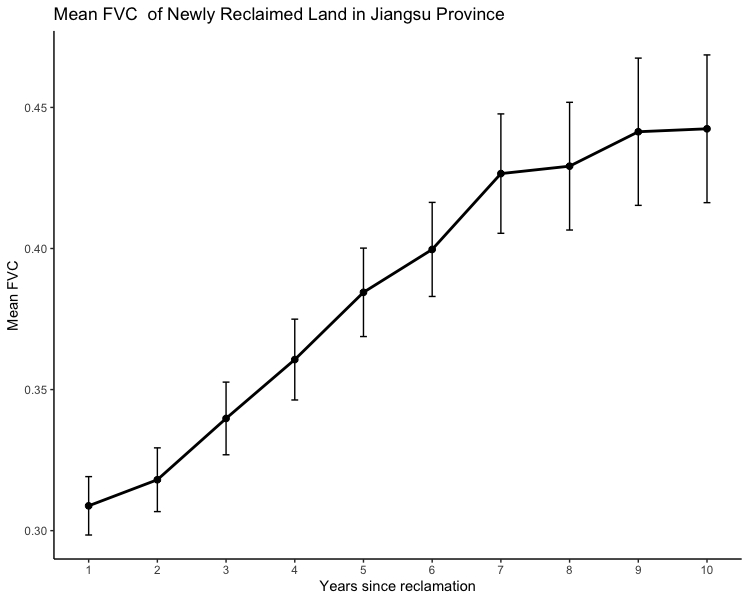
\includegraphics[width=0.8\linewidth]{Motivating_fvc.png}
    \caption{Evolution of Vegetation Coverage after Reclamation}
    \label{fig:fvc}
    \end{figure}

    \begin{figure}[htbp]
    \centering
    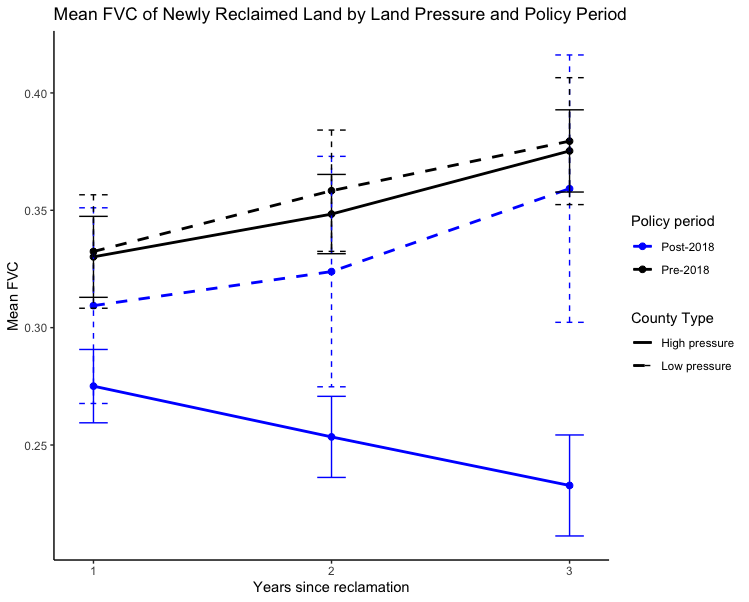
\includegraphics[width=0.8\linewidth]{Motivating_reclaimed_group.png}
    \caption{Vegetation Coverage after Reclamation by Land Protection Pressure and Polity Period}
    \label{fig:fvc_group}
    \end{figure}






\section{Conceptual Framework\label{sec:concept}}
This section lays out a conceptual framework that organizes the institutional setting, clarifies the incentives faced by different agents, and guides the empirical analysis. 
The framework is not intended to solve a formal model, but rather to guide the empirical analysis and to derive testable implications.

\subsection{Land Characteristics and Agricultural Productivity}

Consider a set of land plots indexed by $j$. Each plot is characterized by two fundamental attributes.

First, each plot has an economic potential, denoted by $p_j$, which captures the economic value of converting the plot to construction land. 
This value is determined by access to infrastructure, proximity to urban centers, and other locational advantages, and reflects the contribution of the plot to urban economic growth if developed.

Second, each plot has an intrinsic land quality, denoted by $q_j$. 
Land quality reflects agronomic and biophysical conditions such as soil suitability, slope or ruggedness, drainage, and water availability. 
Importantly, $q_j$ is an exogenous characteristic of the plot and does not depend on current cultivation decisions.

If a plot is converted to cropland, its expected agricultural output depends on both land quality and cultivation effort.
We represent this relationship using a production function:

\begin{equation}
y_j = f(q_j, e_j),
\end{equation}

where $q_j$ denotes intrinsic land quality, $e_j$ represents cultivation effort, including irrigation, planting, and early-stage maintenance, and $y_j$ captures the plot's expected agricultural output.

We assume that higher land quality raises the marginal return to cultivation effort, formally $f_{qe} > 0$. 
Equivalently, for a given level of output, achieving that level requires less effort on higher-quality land. 
This assumption captures a well-established agronomic regularity: improving or cultivating low-quality land is substantially more costly and yields lower returns than cultivating land with favorable natural conditions.

\subsection{Government Objectives and Information Constraints}

The central government seeks to preserve agricultural output through two dimensions: the total area of cropland and its productivity. 
In principle, both dimensions are relevant for food security. 
In practice, however, these two dimensions differ sharply in observability.

Cropland area is directly observable and verifiable through administrative records and satellite imagery. By contrast, land quality, cultivation effort, and agricultural productivity are difficult to monitor, especially at the plot level. As a result, policy enforcement and performance evaluation primarily focus on meeting cropland-area targets, while productivity and actual cultivation outcomes receive far less effective oversight.

Local governments face a different objective function. They are responsible for promoting local economic growth---largely through urban development---and for fulfilling cropland-area mandates imposed by higher levels of government. 
Conditional on meeting the land protection requirements, local governments have incentives to minimize the fiscal and political costs associated with cropland expansion, thereby allocating more resources to growth-enhancing activities. Local governments do not fully internalize agricultural productivity $y_j$, since it is weakly monitored and plays a limited role in economic growth.

\subsection{Land Pressure and Local Trade-offs}

Cities differ in the extent of land-use pressure they face. 
Low-pressure cities possess substantial land reserves that are low in economic potential but high in land quality. 
In these locations, expanding cropland does not require sacrificing valuable urban land or incurring high reclamation costs.

High-pressure cities, by contrast, have limited land reserves overall, which implies that the stock of land that is both low in economic potential and high in agronomic quality is insufficient to meet their cropland-area obligations. When faced with binding cropland-area mandates, local governments in these cities confront a trade-off. 
They can either (i) reclaim low-quality land at relatively low fiscal cost, or (ii) obtain high-quality cropland at substantially higher cost, for example through quota trading or other costly institutional arrangements. Because the second option is considerably more expensive, high-pressure cities rationally choose the first, expanding cropland primarily on low-quality land.

This mechanism implies that, following a tightening of cropland-area regulation, the marginal plots brought into cultivation in high-pressure cities are of lower quality. As a result, average cropland quality deteriorates in locations where land-use pressure is most severe.

\subsection{Farmers' Response and Fallowing}

After land is converted to cropland, cultivation decisions are made by farmers, cooperatives, or agricultural firms. These actors care directly about agricultural productivity $y_j$, not about administrative area targets. 
On low-quality plots, the marginal return to cultivation effort is low, making intensive cultivation unattractive. 
Consequently, such plots may receive little effort or remain uncultivated altogether.

This divergence between local government incentives and farmers' objectives generates a key outcome of the framework: newly reclaimed cropland in high-pressure cities is more likely to exhibit low vegetation cover, poor recovery after reclamation, and a higher probability of fallowing. 

\subsection{Testable Implications}

The framework yields several testable implications that guide the empirical analysis. First, following the policy tightening, plots located in high-pressure cities are more likely to be converted to cropland. Second, newly reclaimed cropland in these cities should be of lower quality, as measured by soil suitability and related indicators. Third, due to weak cultivation incentives, these plots should exhibit lower vegetation cover and higher fallowing rates over time. 
The remainder of the paper evaluates these predictions using high-resolution spatial data on land use, land quality, and vegetation dynamics.


\section{Empirical Analysis\label{sec:empirical}}

\subsection{Identification Strategy}

The empirical analysis exploits cross-county variation in land protection pressure to identify the effects of the 2017 tightening of cropland protection. Land protection pressure is constructed using pre-determined land-use characteristics and administrative constraints, as described in detail in Section~\ref{sec:data}. Intuitively, the national policy tightening constitutes a common shock, while cross-county differences in pressure reflect heterogeneity in how binding the policy is across locations. 

The analysis proceeds in two complementary parts. First, I examine how cropland allocation evolves over time across counties facing different levels of land protection pressure, using an event-study design applied to all grid cells. This approach captures adjustments in cropland area following the policy tightening. Second, I focus on newly reclaimed land and study post-reclamation outcomes using a cohort-based difference-in-differences design. This second approach isolates adjustment along the intensive margin along two dimensions: the suitability of newly created cropland, as proxied by soil characteristics, and its subsequent utilization, as measured by fallow status or vegetation coverage. Together, the two designs allow for a comprehensive assessment of responses to tightened cropland protection along both the extensive and intensive margins.


\subsubsection{Event-Study Design}

To study the effects of the policy tightening on cropland allocation, I estimate a two-way fixed effects event-study specification that interacts land protection pressure with event-time indicators relative to 2017. The unit of observation is a grid cell $i$ located in county $c$ and observed in year $t$. The estimating equation is given by:

\begin{equation}
    \text{cropshare}_{ict}
    =
    \sum_{k \neq -1}
    \beta_k
    \big(
        \text{Pressure}_{c} 
        \times 
        \text{Event}_{k,t}
    \big)
    +
    \mu_i
    +
    \lambda_t
    +
    \varepsilon_{ict},
\end{equation}

where $\text{cropshare}_{ict}$ denotes the share of cropland in grid cell $i$ at time $t$. $\text{Pressure}_{c}$ measures county-level land protection pressure, and $\text{Event}_{k,t}$ is an indicator for event time $k$ relative to the policy tightening in 2017, with $k=-1$ omitted as the reference period. Grid fixed effects $\mu_i$ absorb time-invariant spatial heterogeneity, while year fixed effects $\lambda_t$ control for common shocks affecting all locations. By construction, grid fixed effects also absorb all time-invariant heterogeneity at higher administrative levels, including prefecture- and county-level characteristics.


The coefficients $\beta_k$ trace out how cropland allocation responds over time to the policy tightening as a function of land protection pressure. Identification relies on the assumption that, absent the policy change, cropland trends would have evolved similarly across counties with different levels of land protection pressure.

\subsubsection{Cohort-Based Difference-in-Differences for Newly Reclaimed Land}

While the event-study design captures aggregate changes in cropland allocation, it does not directly address the suitability and subsequent use of newly created cropland. To study post-reclamation outcomes, I exploit variation across reclamation cohorts using a cohort-based difference-in-differences design.

The sample is restricted to grid cells that transition into cropland during the sample period. Each grid cell $i$ is characterized by a reclamation year $t_0(i)$ and is observed for $s$ years after reclamation. The outcome variable $Y_{i,s}$ captures post-reclamation outcomes along two intensive-margin dimensions: the suitability of newly created cropland, as reflected in soil characteristics, and its subsequent utilization, as measured by indicators for fallow status or vegetation coverage.

Treatment intensity is defined as
\begin{equation}
    W_i = \mathbf{1}\{t_0(i) \geq 2018\} \times \text{Pressure}_{c(i)},
\end{equation}
which captures differential exposure to the policy tightening interacted with local land protection pressure. The empirical model is:
\begin{equation}
    Y_{i,s}
    =
    \alpha_{c(i)} 
    + 
    \mu_{t_0(i)}
    +
    \delta_s
    +
    \beta W_i
    +
    X_i'\gamma
    +
    \varepsilon_{i,s},
    \label{mod_cohort}
\end{equation}
where $\alpha_{c(i)}$ are county fixed effects, $\mu_{t_0(i)}$ are reclamation-cohort fixed effects, and $\delta_s$ are years-since-reclamation fixed effects. This specification compares post-reclamation outcomes across grids reclaimed before and after the policy tightening, within counties and relative to common post-reclamation dynamics.

Identification in this design relies on the assumption that, absent the policy tightening, post-reclamation trajectories in both cropland suitability and land-use intensity would have evolved similarly across reclamation cohorts within a county, conditional on land protection pressure. Empirical evidence bearing on this assumption is presented in section~\ref{mainr}.



\subsection{Main Results\label{mainr}}

Figure~\ref{fig:es_cropshare} reports event-study estimates of how grid-level cropland share responds to land protection pressure around the policy change. The pre-policy coefficients are small and statistically indistinguishable from zero, indicating no evidence of differential pre-trends in cropland allocation across counties with different levels of land protection pressure prior to 2017. Following the policy tightening, cropland share increases significantly more in high-pressure counties, with the estimated coefficients turning positive and growing over time. This implies that grids in high-pressure counties are more likely to be converted into cropland after 2017. To facilitate interpretation of the magnitude, I normalize the land protection pressure index to have a standard deviation of one. A one-standard-deviation increase in land protection pressure is associated with a cumulative increase of approximately 0.7 percentage points in grid-level cropland share by 2022, with the gap emerging immediately after the 2017 policy tightening and widening over time.

The next analysis turns to the intensive margin and examines the characteristics of newly reclaimed land. Table~\ref{tab:soil} reports estimates from Model~\ref{mod_cohort}, where the outcome variable measures soil suitability at the time of reclamation. Across specifications using both a continuous soil suitability index and an indicator for land suitable for cultivation (soil suitability $\geq 3$), the interaction between land protection pressure and the post-2017 indicator is negative and statistically significant. These estimates indicate that newly reclaimed land in high-pressure counties after the policy tightening is of lower agronomic quality. Using the binary suitability measure, the coefficient implies that newly reclaimed land in high-pressure counties after 2017 is 5.1 percentage points less likely to be suitable for cultivation, relative to a control mean of 59.6 percent, corresponding to an 8.5 percent increase in the likelihood that newly reclaimed land is unsuitable for agriculture. The results are robust to the inclusion of county-specific time-varying controls interacted with year, which absorb differential local trends. These findings indicate that the tightening of cropland protection is associated with land misallocation along the intensive margin, whereby newly reclaimed cropland in high-pressure regions is drawn disproportionately from land with low inherent suitability for cultivation.





\begin{figure}[htbp]
    \centering
    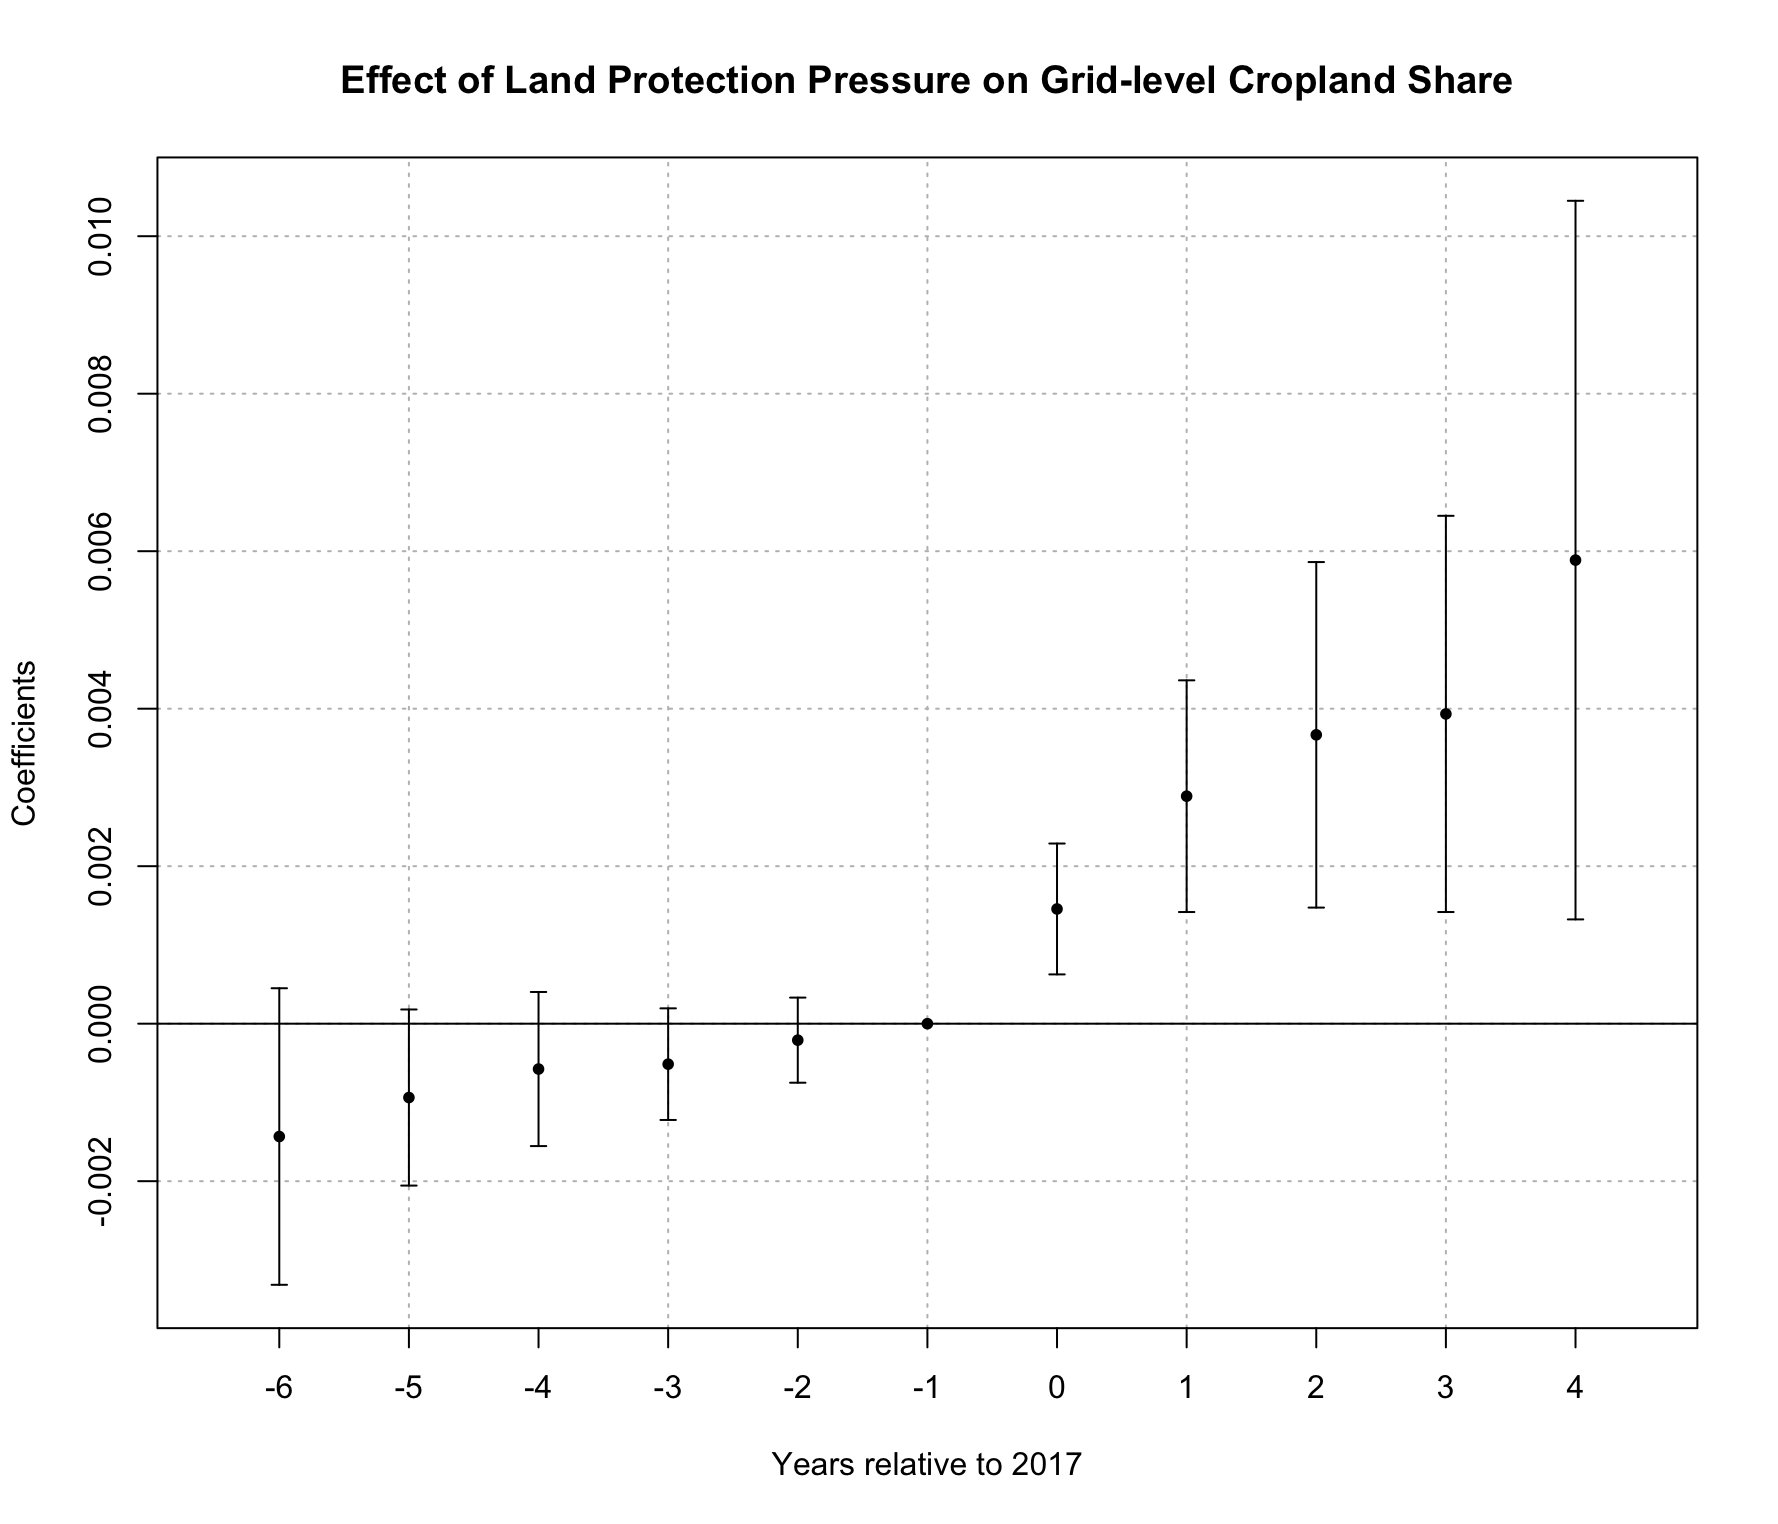
\includegraphics[width=0.8\textwidth]{res_size.png}
    \caption{Effect on Cropland Share}
    \label{fig:es_cropshare}
\end{figure}


\begin{table}[htbp]\centering
\caption{Land Protection Pressure and Soil Suitability of Newly Reclaimed Cropland}
    
\begin{tabular}{lcccc}
\toprule
& \multicolumn{2}{c}{Soil Suitability (1–5)} 
& \multicolumn{2}{c}{Soil Suitability($\geq 3$)} \\
\cmidrule(lr){2-3} \cmidrule(lr){4-5}
& (1) & (2) & (3) & (4) \\
\midrule

Land Protection Pressure × Post 
& -0.183\textsuperscript{***} 
& -0.202\textsuperscript{***} 
& -0.051\textsuperscript{***}  
& -0.051\textsuperscript{***} \\
& (0.058) & (0.064) & (0.018) & (0.017) \\[2pt]

Control Mean
& 3.45 & 3.45 & 0.596 & 0.596 \\

County Controls X Year
&  & $\checkmark$ &  & $\checkmark$ \\

County \& Cohort FE 
& $\checkmark$ & $\checkmark$ & $\checkmark$ & $\checkmark$ \\

Number of Counties
& 52 & 52 & 52 & 52 \\

Num. Obs. 
& 939 & 939 & 939 & 939 \\

R$^{2}$ 
& 0.414 & 0.417 & 0.422 & 0.426 \\

\bottomrule
\end{tabular}




    \label{tab:soil}
    \caption*{\begin{footnotesize}
\textit{Notes}: This table reports cohort-based difference-in-differences estimates from Model~\ref{mod_cohort}. 
The unit of observation is a newly reclaimed grid cell. 
The dependent variable in Columns (1) and (2) is a continuous soil suitability index ranging from 1 (least suitable) to 5 (most suitable). 
The dependent variable in Columns (3) and (4) is an indicator equal to one if soil suitability is greater than or equal to 3, corresponding to land classified as non-saline and suitable for cultivation. 
All specifications include county fixed effects and reclamation-cohort fixed effects. 
Columns (2) and (4) additionally control for county-level time-varying characteristics interacted with year, including population, GDP, government budget, and county area. 
Standard errors are clustered at the county level and reported in parentheses. 
$^{*}p<0.1$, $^{**}p<0.05$, $^{***}p<0.01$.
\end{footnotesize}}
\end{table}

Table~\ref{tab:fallow} reports estimates from Model~\ref{mod_cohort} with fallow status as the outcome variable. Across specifications, the treatment indicator is positive and statistically significant, indicating that newly reclaimed land in high-pressure counties after the policy tightening is more likely to remain fallow. The estimated coefficient implies an increase in the fallow rate of 5.5 percentage points relative to a control mean of 26 percent, corresponding to a 21 percent increase. The results are robust to the inclusion of county-specific time-varying controls interacted with year, as well as county, cohort, and years-since-reclamation fixed effects.

To examine the dynamics of post-reclamation land use, I further interact the treatment variable in Model~\ref{mod_cohort} with years since reclamation and plot the estimated coefficients in Figure~\ref{fig:fallow_dynamic}. The figure shows that the fallow rate in high-pressure counties diverges from that in low-pressure counties as early as the first year after reclamation. This gap persists through at least four years after reclamation, indicating that the increased possibility of fallow is not transitory but sustained over time.



\begin{table}[htbp]\centering
\caption{Land Protection Pressure and Fallow Status of Newly Reclaimed Cropland}
    
\begin{tabular}{lcc}
\toprule
& \multicolumn{2}{c}{Fallow} \\
\cmidrule(lr){2-3}
& (1) & (2) \\
\midrule

Land Protection Pressure × Post 
    & 0.055\textsuperscript{***} 
    & 0.055\textsuperscript{***} \\
& (0.015) & (0.017) \\[2pt]

Control Mean & 0.26 & 0.26 \\

County Controls X Year
    &  
    & $\checkmark$ \\

County \& Cohort FE 
    & $\checkmark$ 
    & $\checkmark$ \\

Year since Reclamation FE
    & $\checkmark$
    & $\checkmark$ \\

Number of Counties
    & 54 & 54 \\

Num. Obs.
    & 3243 & 3221 \\

R$^{2}$
    & 0.230 & 0.229 \\
\bottomrule
\end{tabular}

{\footnotesize
\textit{Notes}: Standard errors in parentheses.
$^{*} p<0.1$, $^{**} p<0.05$, $^{***} p<0.01$.
\par}

    \label{tab:fallow}
\caption*{\footnotesize \textit{Notes}: The table reports cohort-based difference-in-differences estimates from Model~\ref{mod_cohort}. 
The dependent variable is an indicator for whether a newly reclaimed grid cell is fallow in a given post-reclamation year. 
All specifications include county, reclamation-cohort, and years-since-reclamation fixed effects; Column (2) additionally controls for county-level time-varying characteristics interacted with year, including population, GDP, government budget, and county area. 
Standard errors clustered at the county level are reported in parentheses. 
$^{*}p<0.1$, $^{**}p<0.05$, $^{***}p<0.01$.}
\end{table}



\begin{figure}
    \centering   
    \caption{Dynamics of Fallow Status by Years since Reclamation}
    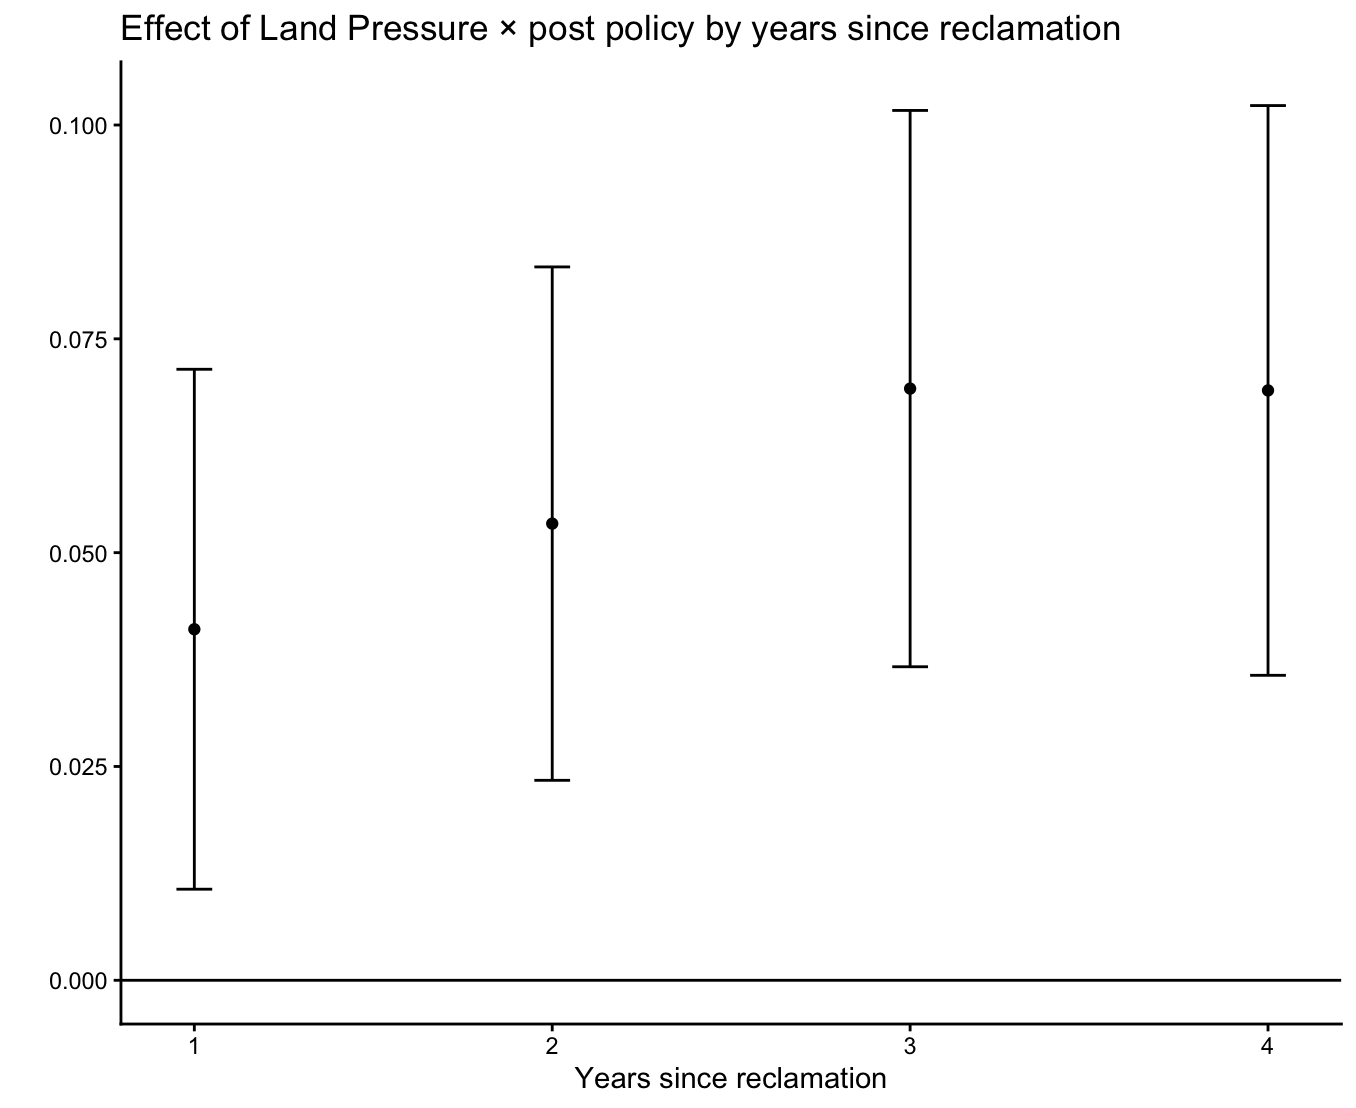
\includegraphics[width=0.7\linewidth]{res_fallow_s.png}
    \label{fig:fallow_dynamic}
    \caption*{\footnotesize \textit{Notes}: The figure plots coefficients from Model~\ref{mod_cohort} interacted with years since reclamation, with 95 percent confidence intervals reported.}
\end{figure}

As a final check on the identifying assumptions, I assess pre-policy trends using a balanced county-level panel of cropland. Pre-trend tests based on newly reclaimed land are not feasible because fallow status is undefined prior to reclamation, and the occurrence of reclamation itself is endogenous to county-year conditions. To circumvent these limitations, I instead examine overall cropland utilization at the county level. Specifically, I aggregate cropland grids to the county-year level and estimate a two-way fixed effects event-study specification using county-level average FVC as the outcome. Figure~\ref{fig:fvc_event} reports the resulting estimates.

Prior to 2017, counties with high and low land protection pressure exhibit similar trends in cropland FVC, providing no evidence of differential pre-trends. After the policy tightening, however, cropland FVC declines significantly more in high-pressure counties relative to low-pressure counties, and this gap persists over subsequent years. These results provide supportive evidence for the identification strategy and indicate that the tightening of cropland protection is associated with lower effective land use in high-pressure counties.



\begin{figure}
    \centering
    \caption{Effect of Land Protection Pressure on County-Level Cropland FVC}
    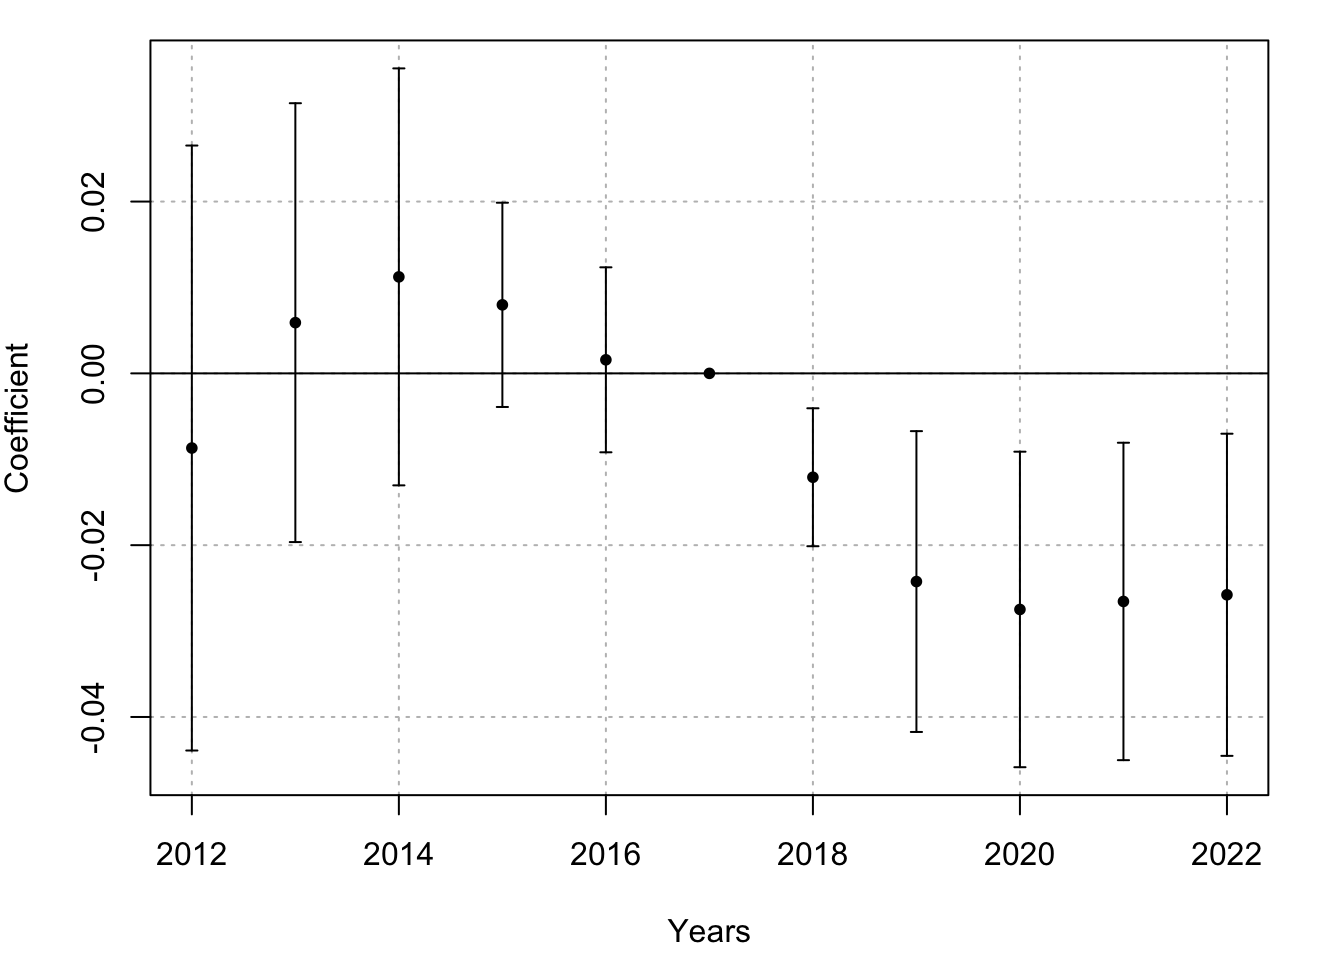
\includegraphics[width=0.75\linewidth]{res_fvc_event.png}
    \caption*{\footnotesize The figure plots coefficients from an event-study specification using county-level cropland data. Cropland is defined as grids with cropland share exceeding 0.6. Bars denote 95 percent confidence intervals.}
    \label{fig:fvc_event}
\end{figure}



\subsection{Mechanisms: Multitask Incentives}

Next, I examine the mechanism underlying the observed patterns in cropland allocation and utilization. The conceptual framework emphasizes multitask incentives faced by local officials, who are simultaneously evaluated on economic growth and cropland protection. When cropland protection targets become binding, officials may seek to satisfy quantitative land requirements at minimal political and fiscal cost, generating distortions in land quality and subsequent land use. Such distortions are expected to be most pronounced when multitask incentives are strongest. I classify counties as being under strong-incentive bureaucrats when the upper-prefecture party secretary satisfies two conditions: (i) they are within the promotion-relevant age window, and (ii) reclamation occurs prior to 2020, a period characterized by high economic growth pressure and limited disruption from COVID-related shocks or nationwide land inspections. Following \cite{huang2024political}, I set age 58 as the promotion cutoff, reflecting the sharp decline in promotion prospects beyond this threshold. Under these conditions, meeting cropland targets while maintaining growth performance is particularly costly, heightening incentives to rely on low-quality land for reclamation.

Table~\ref{tab:mech_incentive} examines whether the deterioration in soil suitability documented in the main results is amplified when multitask incentives are strongest. The baseline effect of land protection pressure after 2017 remains negative and statistically significant. More importantly, the triple interaction between strong incentives, land protection pressure, and the post-policy indicator is also negative and statistically significant across both measures of soil suitability. The estimates show that, conditional on land protection pressure, newly reclaimed land in high-incentive settings exhibits substantially lower agronomic quality. The additional effect associated with strong incentives implies a further reduction in the probability that newly reclaimed land is suitable for cultivation. These findings indicate that binding multitask incentives induce distortions in land allocation, increasing reliance on marginal land to meet cropland protection targets.

To further link land quality to land-use outcomes, I examine the relationship between soil suitability and subsequent fallowing. Table~\ref{tab:mech_soil} shows that newly reclaimed land with lower agronomic quality exhibits significantly higher fallow rates. In particular, grids with low soil suitability are more likely to remain uncultivated after reclamation, reflecting weak incentives to invest in marginal land.

This evidence completes the mechanism connecting multitask incentives to intensive-margin outcomes. When cropland targets are binding under strong multitask incentives, officials are more likely to rely on land with low inherent suitability to satisfy quantitative requirements. Such land is less likely to be cultivated and more prone to fallowing, generating distortions in both land allocation and subsequent land use.



\begin{table}[htbp]\centering 
\caption{Multitask Incentives and Soil Suitability of Newly Reclaimed Land}
\scalebox{0.85}{
\begin{tabular}{lcc}
\toprule
& (1) Soil Suitability (1--5) 
& (2) Soil Suitability ($\geq 3$) \\
\midrule

Pressure $\times$ Post 
& $-0.168$\textsuperscript{***} 
& $-0.046$\textsuperscript{***} \\
& $(0.051)$ & $(0.016)$ \\[0.4em]

Strong Incentive $\times$ Pressure $\times$ Post 
& $-0.089$\textsuperscript{**} 
& $-0.029$\textsuperscript{*} \\
& $(0.043)$ & $(0.014)$ \\[0.4em]

County \& Cohort FE 
& $\checkmark$ & $\checkmark$ \\
Num. Counties 
& 52 & 52 \\
Num. Obs. 
& 939 & 939 \\
R$^{2}$ 
& 0.374 & 0.383 \\
\bottomrule
\end{tabular}}

\label{tab:mech_incentive}
\caption*{\footnotesize
\textit{Notes}: This table reports cohort DID estimates using newly reclaimed cropland data. The dependent variables measure soil suitability at the time of reclamation, using either a continuous index (1–5) or an indicator equal to one if soil suitability is greater than or equal to 3. 
Strong incentives are defined as reclamation occurring when local officials are within the promotion-relevant age window (<58) and prior to 2020, COVID-19. 
All specifications include county and reclamation-cohort fixed effects. 
Standard errors clustered at the county level are reported in parentheses. 
$^{*}p<0.1$, $^{**}p<0.05$, $^{***}p<0.01$.}
\end{table}

\begin{table}[htbp]\centering 
\caption{Soil Suitability and Fallowing of Newly Reclaimed Land}

\scalebox{0.85}{
\begin{tabular}{lcc}
\toprule
& \multicolumn{2}{c}{Outcome: Fallow} \\
\midrule
& (1) Soil Quality (1--5) 
& (2) Soil Quality ($\geq 3$) \\
\midrule

Pressure $\times$ Post 
& $0.099^{***}$ 
& $0.084^{***}$ \\
& $(0.030)$ & $(0.025)$ \\[0.4em]

Soil Suitability $\times$ Pressure $\times$ Post 
& $-0.010^{**}$ 
& $-0.034^{*}$ \\
& $(0.005)$ & $(0.018)$ \\[0.4em]

County, Cohort \& Year FE 
& $\checkmark$ & $\checkmark$ \\
Num. Counties 
& 52 & 52 \\
Num. Obs. 
& 3,185 & 3,185 \\
R$^{2}$
& 0.229 & 0.229 \\
\bottomrule
\end{tabular}}




\label{tab:mech_soil}
\caption*{\footnotesize
\textit{Notes}: This table reports cohort DID estimates using newly reclaimed cropland data.
The dependent variable is an indicator for whether a newly reclaimed grid is fallow in a given post-reclamation year.
All specifications include county, reclamation-cohort, and years-since-reclamation fixed effects. 
Standard errors clustered at the county level are reported in parentheses. 
$^{*}p<0.1$, $^{**}p<0.05$, $^{***}p<0.01$.}
\end{table}

\subsection{Robustness Checks}

I conduct a series of robustness checks to assess the sensitivity of the main results to alternative definitions of key variables and sample constructions. First, I examine whether the findings depend on how land protection pressure is measured. I consider alternative constructions of the pressure index by (i) redefining core-urban districts in the obligation component and (ii) modifying the definition of available land in the total-land component. These exercises test whether the results are driven by specific coding choices in the pressure measure.

Second, I evaluate the sensitivity of the results to the classification of newly reclaimed land and fallow status. I vary the threshold used to define reclamation based on pre-reclamation cropland share and allow for a range of alternative cutoffs. I also consider alternative definitions of fallow land by varying the FVC threshold used to identify uncultivated plots. All robustness exercises are implemented for the main outcomes and are reported in the Appendix.


\section{Discussion and Conclusion\label{sec:conclude}}
This paper examines how tighter enforcement of cropland protection shapes local land-use behavior in a centralized administrative system characterized by multitask incentives and imperfect monitoring. Leveraging cross-county differences in exposure to cropland protection pressure, the analysis shows that the post-2017 policy tightening generates responses along both the extensive and intensive margins of land use. Counties subject to higher pressure are more likely to expand cropland area, yet the land brought into cultivation is of lower soil suitability and is cultivated less intensively, with elevated fallow rates that persist over time. These patterns suggest that stricter enforcement of observable quantity targets can induce distortions in land allocation and land use when monitoring of land quality and utilization remains limited.

The consequences of these distortions extend beyond short-run mismatches between land endowments and land-use categories. The reclamation of marginal or low-quality land weakens agricultural productivity not only through inferior land characteristics but also through reduced cultivation intensity, higher abandonment, and inefficient input use. Over time, these channels translate into economic losses that are not reflected in aggregate cropland area statistics. As a result, policies that succeed in stabilizing cropland quantity may nevertheless fail to achieve broader productivity objectives if they redirect land use toward plots with limited productive potential.

The findings also inform the design of policy implementation. A common response to execution distortions is to strengthen monitoring to additional dimensions, such as land quality and utilization, yet this approach may be constrained by administrative capacity. This study instead highlights the role of institutional arrangements, particularly the restricted functioning of cropland quota markets. Because cropland replenishment indicators do not circulate freely across prefectures, local governments facing binding targets have limited adjustment margins beyond local land reclamation. Greater flexibility and integration in cropland indicator markets would enlarge the set of feasible compliance options, reducing the likelihood that multitask pressure results in distortive implementation. More broadly, the results underscore that mitigating misallocation under multitask governance requires not only tighter oversight, but also institutional designs that align incentives with policy objectives under realistic monitoring constraints.


\bibliography{../Bibliography_base}

\newpage

\appendix
\section{Additional Results and Robustness Checks}
\begin{table}[ht!]
\centering
\footnotesize
\caption{Robustness: Alternative Definitions of Land-Pressure Exposure}
\begin{tabular}{lccc}
\toprule
 & (1) Cropland Share & (2) Soil Suitability $\ge 3$ & (3) Fallow \\ 
\midrule
\multicolumn{4}{l}{\textbf{Panel A: All Land Types as Available Land}} \\
Pressure $\times$ Post 
  & $0.006^{***}$ & $-0.074^{***}$ & $0.078^{***}$ \\
  & $(0.002)$ & $(0.023)$ & $(0.026)$ \\[0.6em]

\multicolumn{4}{l}{\textbf{Panel B: Alternative Definition of Core-Urban Districts}} \\
Pressure $\times$ Post 
  & $0.003^{**}$ & $-0.048^{*}$ & $0.084^{**}$ \\
  & $(0.002)$ & $(0.026)$ & $(0.032)$ \\

\bottomrule
\end{tabular}

\vspace{0.5em}
{\footnotesize
$^{***} p<0.01$,
$^{**} p<0.05$,
$^{*} p<0.10$.
\par}

\caption*{\footnotesize 
\textit{Notes}: This table examines the robustness of the main results to alternative definitions of land-protection pressure. 
In Panel A, \textit{available land} is redefined to include all land types, rather than excluding water bodies and impervious surfaces as in the baseline specification. 
In Panel B, the classification of \textit{core-urban districts} is tightened by coding only fully core districts as core, while partially core districts are grouped with non-core districts. 
All specifications otherwise follow the baseline empirical design.}
\end{table}


\begin{figure}[ht!]
    \centering
    \caption{Sensitivity to Alternative Thresholds in Reclaimed-Land Definition: Fallow}
    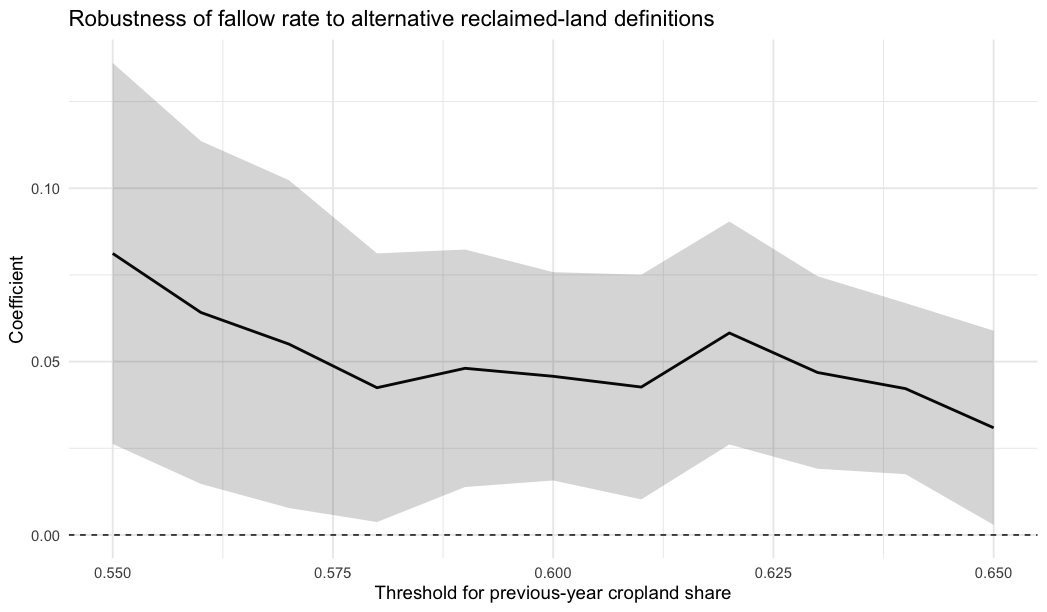
\includegraphics[width=0.8\linewidth]{sensitivity_fallow_lowbound0.6.png}
\end{figure}

\begin{figure}[ht!]
    \centering
    \caption{Sensitivity to Alternative Thresholds in Reclaimed-Land Definition: Soil Suitability}
    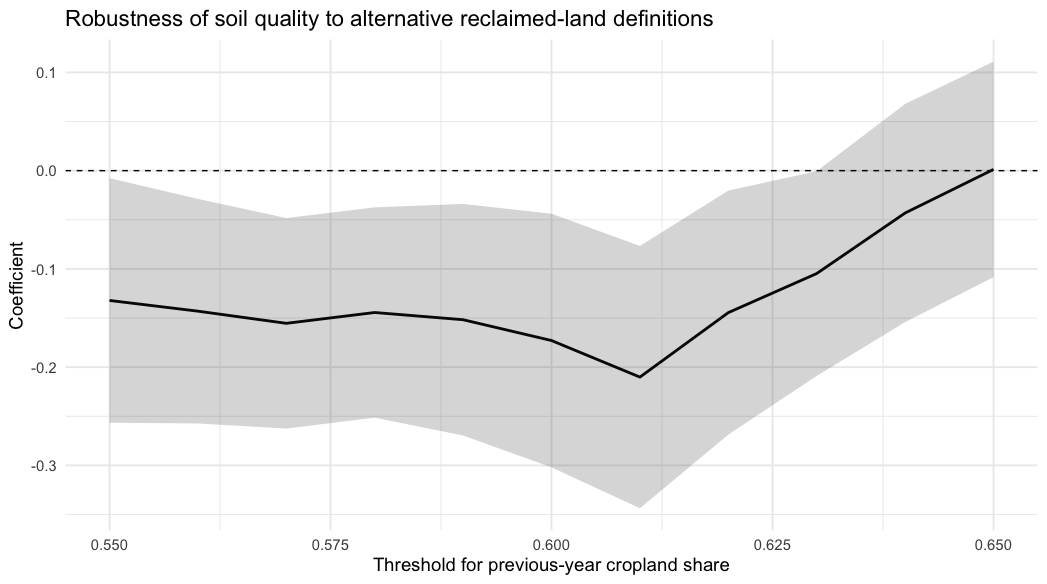
\includegraphics[width=0.8\linewidth]{sensitivity_soil.png}
\end{figure}


\begin{figure}
    \centering
    \caption{Sensitivity to Alternative Fallow Rate Definition}
    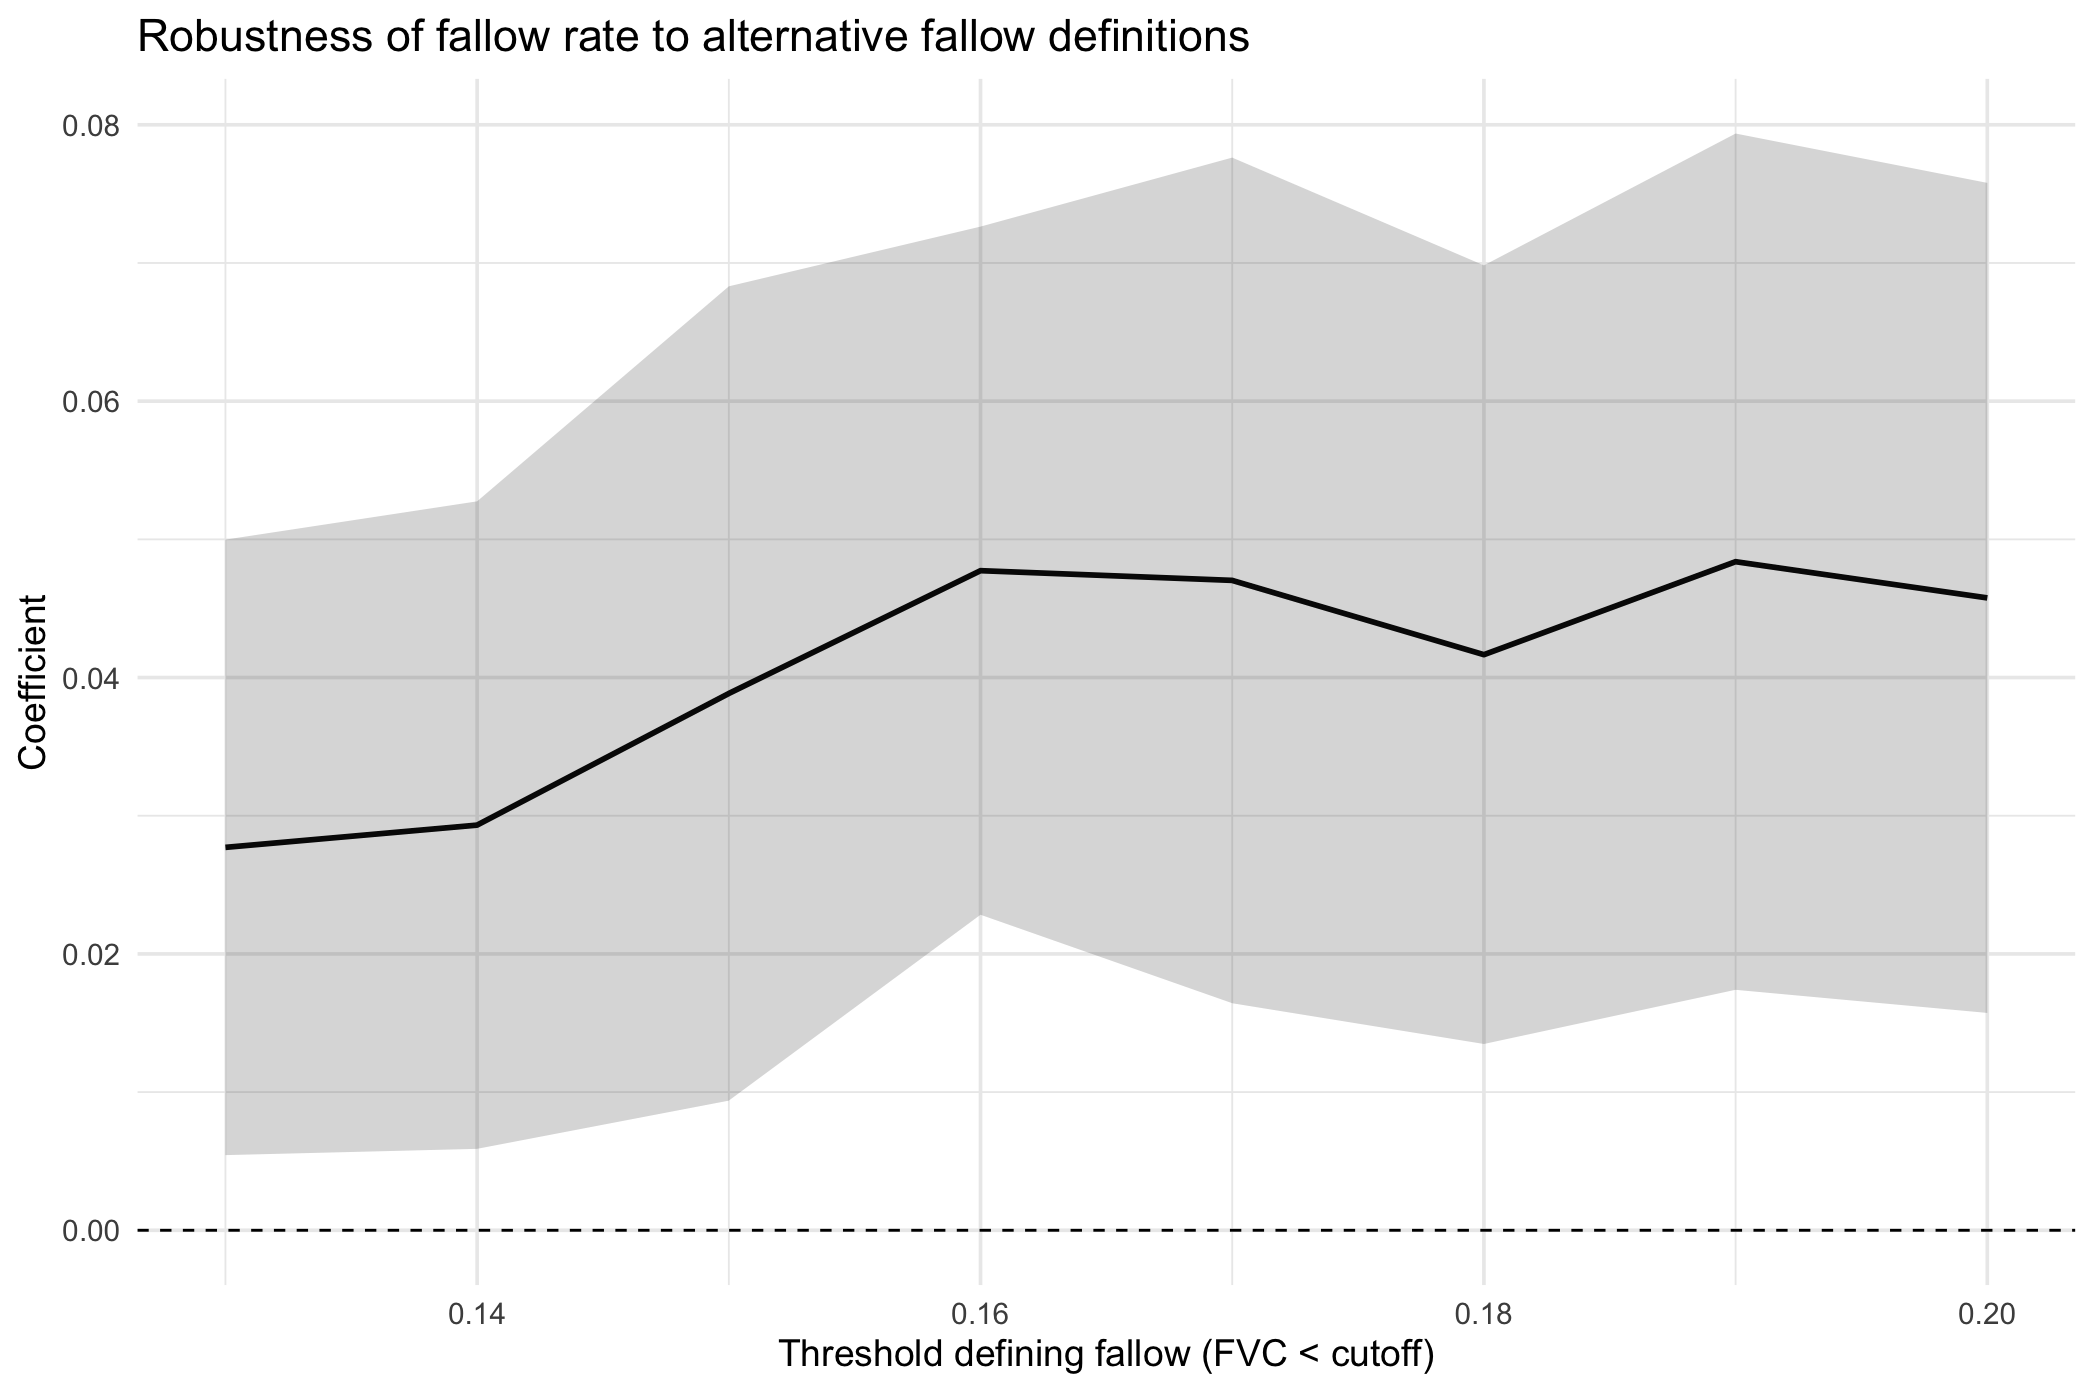
\includegraphics[width=0.8\linewidth]{sensitivity_fallow_rate0.2.png}
    \label{fig:sensitivity_fallow02}
\end{figure}




\end{document}
